\documentclass[aps,prl,reprint,twocolumn,amsmath,amssymb,floatfix,nofootinbib,superscriptaddress]{revtex4-2}
\usepackage{amsmath,amssymb,amsthm,booktabs,graphicx,hyperref}
\usepackage{tikz,pgfplots}
\pgfplotsset{compat=1.18}
\usetikzlibrary{arrows.meta,calc,positioning,decorations.pathreplacing}
% Sans-serif maths for the figures: Helvetica digits and roman, sans-italic letters (newtxsf)
\DeclareMathVersion{figsans}
\SetSymbolFont{operators}{figsans}{OT1}{phv}{m}{n}
\SetSymbolFont{letters}{figsans}{OML}{ntxsfmi}{m}{it}
\SetSymbolFont{symbols}{figsans}{OMS}{cmsy}{m}{n}
\SetMathAlphabet{\mathrm}{figsans}{OT1}{phv}{m}{n}
\SetMathAlphabet{\mathbf}{figsans}{OT1}{phv}{b}{n}
\hypersetup{hidelinks}
\newtheorem{theorem}{Theorem}
\newtheorem{lemma}[theorem]{Lemma}
\newtheorem{proposition}[theorem]{Proposition}
\newtheorem{corollary}[theorem]{Corollary}
\theoremstyle{definition}
\newtheorem{definition}[theorem]{Definition}
\theoremstyle{remark}
\newtheorem{remark}[theorem]{Remark}
\newcommand{\F}{\mathbb F_2}
\newcommand{\CCZ}{\mathrm{CCZ}}
\newcommand{\CS}{\mathrm{CS}}
\newcommand{\tr}{\operatorname{Tr}}
\newcommand{\wt}{\operatorname{wt}}
\newcommand{\fs}{\mathbb V}
\newcommand{\Z}{\mathbb Z}
\begin{document}
\title{Cultivating Magic States Without Losing Distance}
\author{Lloren\c{c} Balada Gaggioli}
\affiliation{Czech Technical University in Prague, Prague, Czech Republic}
\affiliation{LAAS-CNRS, Universit\'e de Toulouse, France}
\author{Jakub Mare\v{c}ek}
\affiliation{Czech Technical University in Prague, Prague, Czech Republic}
\date{Draft, \today}
\begin{abstract}
Magic-state cultivation is a leading way to make the T states that fault-tolerant quantum computers need. Its circuits are designed and tested in simulations that replace every T gate by an S gate, because only then can they be simulated efficiently. We show that this shortcut hides a real loss. An exact criterion reduces any cultivation circuit to one stabilizer code on its T gates, and it reveals that current cultivation circuits, including the one run on Google's hardware, tolerate only about half the faults their simulations promise. We trace the loss to a simple mechanism and design checks that avoid it. On a square grid with nearest-neighbour gates, they keep the full fault tolerance and fail a thousand times less often than the checks of the experiment.
\end{abstract}
\maketitle

%
\section{Introduction}
A fault-tolerant quantum computer needs a supply of T states, $|T\rangle=(|0\rangle+e^{i\pi/4}|1\rangle)/\sqrt2$, because the gates that error-correcting codes implement easily, the Clifford gates, are not universal on their own. Magic-state cultivation~\cite{cultivation} is one of the most economical ways known to make them. It prepares a T state in a small color code and then checks it repeatedly, keeping the state only when every check passes. The checks use physical T gates. Simulations predict that cultivation reaches logical error rates that previously required distillation, at a cost comparable to a single logical CNOT~\cite{cultivation}, and Google has demonstrated it on a superconducting processor~\cite{googlecultivation}.

There is a catch in how these circuits are designed. A circuit of Clifford gates can be simulated efficiently, but a circuit with T gates cannot. Cultivation circuits are therefore simulated with every T gate replaced by an S gate, its Clifford square. We call this the S proxy. The proxy keeps the structure of every check, and its simulations decide the circuits that are proposed and built. Recent exact simulations with real T gates show that the proxy is not faithful: the distance-three and distance-five circuits of Ref.~\cite{cultivation} tolerate fewer faults than their proxies~\cite{chan,wanzapirain}. This raises three questions. Is there a criterion that decides fault tolerance with real T gates, for every circuit? How much do circuits lose in general, and why? And can a check keep all of it?

We answer all three. First, the fault tolerance of any cultivation circuit is decided by one stabilizer code on its T gates together with a linear map from faults to Pauli errors on those T gates. Because the checks of cultivation are deterministic, this criterion has an exact closed form that a computer evaluates in polynomial time. Second, with this criterion we find that current checks lose about half their distance: a circuit that the proxy says tolerates any $d-1$ faults tolerates only $(d-1)/2$ with real T gates, at code distances three, five and seven, and the circuit of Google's experiment is one of them. The loss has a single cause, which we identify. Third, a check that avoids this cause keeps the full distance, and it fits on a square grid with nearest-neighbour gates, where it is also cheaper than the checks in use today.

%
\section{Cultivation and fault distance}
A cultivation circuit starts by injecting a T state into a color code, a quantum error-correcting code whose logical qubit is protected against errors on fewer than half of its code distance $\delta$ physical qubits. It then checks the logical state. A check applies a T gate to every data qubit, measures the logical X operator, and undoes the T gates. This measures $TXT^\dagger$, of which $|T\rangle$ is an eigenstate, so a correct T state passes every check, and a state that fails is discarded. Finally an ideal decoder reads out the code: it measures all stabilizers, keeps the state only if none is violated, and unencodes the logical qubit. This last step stands for the later stages of a real protocol, where the code is grown and protected by error correction. Fig.~\ref{fig:small}(a) shows on the Bloch sphere what a single check does to an error.

Every operation of the circuit is noisy. We model a fault as a Pauli error after a preparation or a gate, or as a wrong measurement outcome, with each location failing independently with probability of order $p$. A configuration of faults is \emph{harmless} if the circuit then either rejects the state or outputs the correct one, and \emph{harmful} if it accepts a wrong state. The \emph{fault distance} $d$ is the smallest number of faults that can be harmful, so that the error of an accepted state scales as $p^d$. The fault distance cannot exceed the code distance $\delta$, since $\delta$ errors on the data at the end of the circuit can form an undetectable logical error (Sec.~\ref{sm:proofs}). A circuit with $d=\delta$ keeps its full distance.

%
\section{One code decides}
The main obstacle to analysing the circuit exactly is that a Pauli fault before a T gate becomes a non-Pauli error after it. We move the T gates out of the way. A T gate on a qubit can be replaced by a small Clifford circuit that consumes an ancilla prepared in $|T\rangle$: a CNOT from the qubit to the ancilla, followed by a projection of the ancilla onto $|0\rangle$~\cite{zhouleungchuang},
\begin{equation}
 \sqrt2\,\langle0|_a\,\mathrm{CX}_{q\to a}\,|\psi\rangle_q|T\rangle_a=T|\psi\rangle_q .
 \label{eq:gadget}
\end{equation}
Doing this for all $t$ T gates leaves a noisy Clifford circuit, the \emph{skeleton}, that acts on $t$ ideal T states. A Clifford circuit can be followed exactly with the stabilizer formalism. Each fault can be pushed to the end of the skeleton, where it either contradicts a measurement outcome that is fixed in the skeleton, which we call a \emph{detector}, or acts as a Pauli error on the $t$ T-state inputs.
\begin{theorem}\label{thm:main}
Let a cultivation circuit with $t$ T gates, without feedforward and with every measurement postselected, prepare a target state $\tau$ when no fault occurs, where no Pauli operator other than the identity fixes $\tau$, as for a T state. There are a stabilizer code $C$ on $t$ qubits and two linear maps, $D$ from fault configurations to detector patterns and $E$ from fault configurations to Pauli operators on $t$ qubits, defined up to phases and the stabilizers of $C$, such that a fault configuration $F$ is harmless if and only if $D(F)\neq0$ or
\begin{equation}
 \Pi_C\,E(F)\,|T\rangle^{\otimes t}\in\mathbb C\,\Pi_C|T\rangle^{\otimes t},
 \label{eq:collapse}
\end{equation}
where $\Pi_C$ is the projection onto the code $C$.
\end{theorem}
In words: a fault configuration is harmless exactly when it is detected, or when the code $C$ still projects the perturbed T states onto the correct encoded state, or onto zero. The code $C$ does not depend on the faults. It is fixed by the circuit, and the faults only choose which Pauli operator $E(F)$ perturbs its inputs. Eq.~\eqref{eq:collapse} is the same condition that decides magic-state distillation, where perfect Clifford circuits measure a code on noisy T states~\cite{distillationpaper}. Cultivation differs only in the linear map $E$, which carries faults from anywhere in the circuit onto the T states. The pair $(D,E)$ plays the role that the detector error model plays for Clifford circuits~\cite{stim}. Protocols with feedforward and random choices reduce to the circuit of one accepted run without loss of fault distance (Proposition~\ref{prop:branch}), and the proofs are in Sec.~\ref{sm:proofs}.

\paragraph*{An exact test.}
The condition~\eqref{eq:collapse} involves the state $|T\rangle^{\otimes t}$, whose dimension grows exponentially. In cultivation it can be decided without ever writing this state down. The reason is that every check is deterministic on the target: a Z error on the T gates commutes with them, so it either leaves the state in the code, flips the logical qubit, or is rejected with certainty. An X error is different, because $X|T\rangle=(|T\rangle+iZ|T\rangle)/\sqrt2$ is a superposition of a correct and a Z-flipped T state. A Pauli error with an X part on $|a|$ inputs therefore spreads over $2^{|a|}$ Z patterns, and the code sorts each of them into the correct state, the wrong state, or rejection. Adding up the amplitudes gives the following result, with the precise statement and proof in Sec.~\ref{sm:gauss}.
\begin{theorem}\label{thm:gauss}
If the checks of the circuit are deterministic, then for every fault configuration $F$ with $D(F)=0$ there are two numbers $g_0(F)$ and $g_1(F)$, each a sum $\sum_z i^{q(z)}$ of powers of $i$ over a quadratic form $q$ with values modulo four, such that $F$ is accepted with probability $2^{-|a|}(|g_0|^2+|g_1|^2)$ relative to the fault-free circuit and outputs a wrong state with probability $2^{-|a|}|g_1|^2$. In particular $F$ is harmful if and only if $g_1(F)\neq0$, and this is decided with $O(t^3)$ operations.
\end{theorem}
Sums of this kind, Gauss sums, are evaluated by eliminating one variable at a time, and each step either multiplies the sum by a simple factor or shows that it vanishes. Every fault configuration of a cultivation circuit can thus be judged exactly, with real T gates, at the cost of linear algebra. We combine this with a stim detector error model of the skeleton, which lists all fault classes with their detector patterns~\cite{stim}, and with a search for sets of faults whose detector patterns cancel. This certifies fault distances as fast as for Clifford circuits. A second, independent implementation, which follows the skeleton symbolically and decides Eq.~\eqref{eq:collapse} with state vectors, agrees on every circuit small enough for both (Secs.~\ref{sm:compute} and~\ref{sm:algorithm}).

\paragraph*{The cost in T gates.}
Theorem~\ref{thm:main} also bounds what cultivation can cost. Z faults on the T gates themselves are never detected and act on the code $C$ exactly like noise on the inputs of a distillation protocol. A circuit of fault distance $d$ therefore contains a distillation protocol of order $d$, and conversely every such protocol can be turned into a cultivation circuit of the same fault distance (Sec.~\ref{sm:distill}).
\begin{theorem}\label{cor:exact}
The least number of T gates in a cultivation circuit of fault distance $d$ for one T state equals the least number of noisy inputs of a distillation protocol of order $d$. It is at least $3d-4$ for odd $d$ and $3d-6$ for even $d$.
\end{theorem}
Fault distance two thus needs exactly nine T gates, and we give a circuit that attains this (Sec.~\ref{sm:t9}). For the larger distances that matter in practice, the number of T gates is not what limits cultivation. The checks are.

%
\section{Real T gates halve the distance}
Every smallest harmful fault configuration we found has the same structure, and the following lemma describes it. Consider a color code of distance $\delta$ and a set $\ell$ of $\delta$ data qubits that carries a logical X operator.
\begin{lemma}[Coherent completion]\label{lem:completion}
Suppose that undetected faults leave an X error on a nonempty proper part $u$ of $\ell$ just before the last layer of T gates, that $u$ contains the support of no Z stabilizer, and that further faults put X on the rest of $\ell$ after it. Then the ideal decoder accepts with probability $2^{-|u|}$ relative to the fault-free circuit and outputs a wrong state. With S gates in place of T gates, the same faults are detected.
\end{lemma}
The reason is that a T gate turns an X error into a superposition, $TXT^\dagger\propto(I-iZ)X/\sqrt2$, as shown in Fig.~\ref{fig:small}(a). After the last T layer the error on $u$ is a superposition of $X^u$ with all Z errors inside $u$. The decoder rejects every component with a Z error, because such an error is too light to be a stabilizer, but it keeps the one component without, and the remaining faults complete $X^u$ to a logical operator. The S gate instead turns X into the Pauli Y, whose Z part the decoder always detects. The proof is in Sec.~\ref{sm:proofs}. A check keeps its full distance only if no $s$ undetected faults can put X on more than $s$ qubits of such a logical set before the last T layer (Sec.~\ref{sm:mechanism}).

Current checks violate this. They measure the logical operator with a GHZ fold: a tree of CNOTs that collects the parity of the data onto one qubit, which is measured, after which the tree is undone. A single X fault on a qubit of the tree spreads, when the tree is undone, to a whole branch of data qubits. With S gates the decoder detects such spreading, but with T gates it is completed coherently (Fig.~\ref{fig:gsj}). We certified this loss on the published circuits, on fold checks that we built at larger distance, and on the circuit of the experiment.
\begin{proposition}[computer-assisted]\label{prop:gsj}\label{prop:fold}\label{prop:google}
With real T gates in place of the S gates of their simulations, (i) the distance-three and distance-five cultivation circuits of Ref.~\cite{cultivation} have fault distance two and three, while their proxies have three and five, (ii) GHZ-fold checks of the same kind on color codes of distance three, five and seven have fault distance two, three and four, for every fold tree we tried, and (iii) the circuit of Google's experiment~\cite{googlecultivation} has fault distance two, while its proxy has three, whether or not its injection is noisy.
\end{proposition}
In every case the fault distance with real T gates is $(\delta+1)/2$, about half the code distance, and the loss grows with the code (Fig.~\ref{fig:fd}). The failures are, however, rare: by Lemma~\ref{lem:completion} they are accepted only with probability $2^{-|u|}$, and the leading term of the logical error of the distance-three circuit of Ref.~\cite{cultivation} is $32p^2/75$, which agrees with the exact series of Ref.~\cite{wanzapirain}. For the experiment, the leading term is $2.2\,p^2$ under SI1000 noise, a standard model of superconducting hardware in which two-qubit gates fail with probability $p$, measurements with $5p$ and single-qubit gates with $p/10$, and which the authors used in their own simulations~\cite{si1000}. At their noise strength, $p=2.3\times10^{-3}$, the logical error of the accepted states is $2.4\times10^{-5}$ with real T gates instead of the $6.9\times10^{-6}$ that the proxy predicts, and the gap grows as $p$ falls, to a factor six at $p=10^{-3}$ (Fig.~\ref{fig:nn}c). The details of all circuits are in Secs.~\ref{sm:gsj} to~\ref{sm:google}, including flags that partly repair the fold (Sec.~\ref{sm:gsj}).

\begin{figure}[t]
\centering
% Figure 2 of cultivation.tex, written by scripts/make_fig_cultivation.py. Requires tikz and pgfplots.
\definecolor{tolblue}{cmyk}{1,0.36,0,0.30}      % T states, absorbed faults
\definecolor{skyblue}{cmyk}{0.63,0.23,0,0.09}   % code, trivial faults
\definecolor{harmver}{cmyk}{0,0.56,1,0.165}     % faulty states, harmful faults
\definecolor{rejgray}{cmyk}{0,0,0,0.62}         % rejected
\definecolor{inkgray}{cmyk}{0,0,0,0.75}         % annotation
\definecolor{pauX}{cmyk}{0,0.31,1,0.10}         % X
\definecolor{pauY}{cmyk}{1,0,0.27,0.38}         % Y
\definecolor{pauZ}{cmyk}{0,0.41,0.18,0.20}      % Z

\begin{tikzpicture}[
  font=\fontsize{8}{9.6}\fontfamily{phv}\selectfont\mathversion{figsans},
  line width=0.5pt,
  >={Stealth[length=1.6mm,width=1.2mm]},
  letter/.style={font=\fontsize{8}{9.6}\fontfamily{phv}\fontseries{b}\selectfont, anchor=north west, inner sep=0pt},
  small/.style={font=\fontsize{7}{8.4}\fontfamily{phv}\selectfont\mathversion{figsans}},
]
\node[letter] at (0,3.05) {(a)};
\begin{scope}[shift={(0.55,-3.55)}, scale=0.78]
\fill[pauX!14] (0.35,4.75) -- (2.15,4.75) -- (2.15,5.79) -- (1.25,6.31) -- cycle;
\fill[pauY!14] (2.15,4.75) -- (3.95,4.75) -- (3.05,6.31) -- (2.15,5.79) -- cycle;
\fill[pauZ!14] (1.25,6.31) -- (2.15,5.79) -- (3.05,6.31) -- (2.15,7.87) -- cycle;
\draw[inkgray] (0.35,4.75) -- (3.95,4.75) -- (2.15,7.87) -- cycle;
\draw[inkgray] (2.15,4.75) -- (2.15,5.79) -- (1.25,6.31) (2.15,5.79) -- (3.05,6.31);
\draw[harmver, line width=1.6pt, line cap=round, opacity=0.55] (0.35,4.75) -- (2.15,7.87);
\fill (0.35,4.75) circle (1.5pt);
\fill (3.95,4.75) circle (1.5pt);
\fill (2.15,7.87) circle (1.5pt);
\fill (2.15,4.75) circle (1.5pt);
\fill (1.25,6.31) circle (1.5pt);
\fill (3.05,6.31) circle (1.5pt);
\fill (2.15,5.79) circle (1.5pt);
\draw[fill=white] (-0.07,5.28) rectangle (0.13,5.48);
\draw[->, harmver, dashed, line width=0.5pt] (1.19,6.27) to[out=200, in=60] (0.13,5.47);
\draw[->, harmver, dashed, line width=0.5pt] (0.03,5.27) to[out=-80, in=150] (0.31,4.81);
\node[anchor=north, inner sep=1.5pt, small] at (0.35,4.75) {1};
\node[anchor=south east, inner sep=1.5pt, small] at (1.25,6.31) {2};
\node[anchor=east, inner sep=1.5pt, small] at (2.15,7.87) {3};
\node[star, star points=6, star point ratio=2.4, fill=harmver, draw=white, line width=0.3pt, inner sep=0pt, minimum size=2.8mm] at (1.55,6.41) {};
\node[star, star points=6, star point ratio=2.4, fill=harmver, draw=white, line width=0.3pt, inner sep=0pt, minimum size=2.8mm] at (2.45,7.87) {};
\node[harmver, anchor=south east, inner sep=1pt] at (1.37,6.68) {$\bar X$};
\end{scope}
\node[letter] at (3.85,3.05) {(b)};
\begin{axis}[at={(4.95cm,0.62cm)}, anchor=south west, width=3.35cm, height=2.2cm, scale only axis,
  xmin=-0.4, xmax=10.5, ymin=0, ymax=3.0, xtick={0,5,10}, ytick={0,1,2,3},
  tick label style={font=\fontsize{8}{9.6}\fontfamily{phv}\selectfont}, label style={font=\fontsize{8}{9.6}\fontfamily{phv}\selectfont\mathversion{figsans}},
  xlabel={$p$ ($10^{-3}$)}, ylabel={$(\epsilon_T-\epsilon_S)/p^2$},
  axis line style={line width=0.5pt}, tick style={line width=0.5pt}, xlabel shift=-3pt, ylabel shift=-4pt,
  clip=false]
\addplot[inkgray, dashed, line width=0.5pt, domain=0:5.6] {0.4448 + 0.146993*x};
\addplot[only marks, mark=*, mark size=1.3pt, black, error bars/.cd, y dir=both, y explicit, error bar style={line width=0.5pt}] coordinates {(1.000,0.5836) +- (0,0.0631) (2.000,0.7468) +- (0,0.0455) (3.000,0.8757) +- (0,0.0768) (5.000,1.1778) +- (0,0.1329) (7.000,1.4206) +- (0,0.2079) (10.000,2.4351) +- (0,0.3566)};
\addplot[only marks, mark=diamond*, mark size=2.4pt, harmver] coordinates {(0,0.4267)};
\end{axis}
\end{tikzpicture}

\caption{How real T gates lose distance in the distance-three circuit of Ref.~\cite{cultivation}. (a)~One of its $48$ harmful pairs of faults, on the seven data qubits of the color code (faces shaded), following Ref.~\cite{chan}. Fault~1, an X error on qubit~2, is copied to qubit~1 through the fold. With S gates the errors become $Y_1Y_2$, which the top face detects. With T gates the component $X_1X_2$ survives, and fault~2 on qubit~3 completes the logical operator $\bar X$ along the left edge. (b)~Difference of the logical errors per accepted run with T and with S gates, divided by $p^2$, from the state-vector simulations published with the circuit~\cite{gsjcode} (one standard deviation, dashed line a weighted linear fit), and its limit $32/75$ at $p\to0$ from Theorem~\ref{thm:main}.}
\label{fig:gsj}
\end{figure}

\begin{figure}[t]
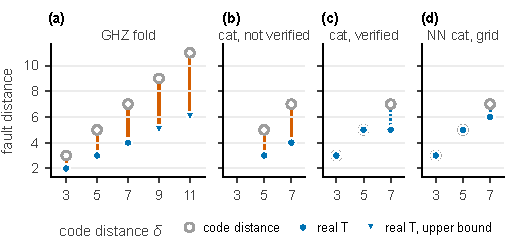
\includegraphics[width=\columnwidth]{fig_fd.pdf}
\caption{Fault distance with real T gates (filled) against the code distance (open), which the S proxy reaches. The vermillion gaps are the distance lost to real T gates. (a)~GHZ folds, including the circuits of Ref.~\cite{cultivation}. (b), (c)~Cat-state checks without and with verification. (d)~Nearest-neighbour cat checks on a square grid. At $d=7$ the verified cats are certified to at least five and six, and the dotted range is open.}
\label{fig:fd}
\end{figure}

%
\section{Keeping the distance}
Lemma~\ref{lem:completion} suggests the remedy: let every data qubit interact with the check only once, through a qubit that no single fault can corrupt together with another. A Shor-style check~\cite{shor} does this. It prepares a cat state $(|0\cdots0\rangle+|1\cdots1\rangle)/\sqrt2$ on fresh qubits, verifies it by measuring parities of its qubits before it touches the data, couples each cat qubit to one data qubit by a CNOT, and reads the check outcome from the parity of the cat qubits in the X basis. A fault in the preparation that spreads X over several cat qubits is caught by the verification, and every other fault reaches at most one data qubit.

Such a check needs no all-to-all connectivity. On a square grid, we grow the cat along a path of qubits from its middle outward, one CNOT per step in each direction, so a single X fault on a path qubit spreads only towards the end of the path beyond it. The parity of the two ends, measured through an ancilla next to both, then catches every such spread. Each data qubit sits next to its own path qubit. After the coupling we undo the growth, so that the outcome sits on one qubit and the other path qubits return to $|0\rangle$, where measuring them gives further checks. At $d=3$ the path runs around a rectangle and the ancilla closes it. At $d=5$ the path folds into a U on three rows, and the middle row measures the parities across the U and along its diagonals, which together catch every spread from two faults (Fig.~\ref{fig:nn}).
\begin{proposition}[computer-assisted]\label{prop:vcat}\label{prop:nn}
Checks with a verified cat keep the full fault distance with real T gates: five on the distance-five color code and at least five on the distance-seven code with all-to-all connectivity, where the same checks without verification have three and four. With nearest-neighbour gates on a square grid, the ring check on the distance-three code ($17$ qubits) and the ladder check on the distance-five code ($46$ qubits) have fault distance three and five, and the ladder on the distance-seven code ($91$ qubits) has at least six.
\end{proposition}
These checks are also cheap. Under SI1000 noise at $p=10^{-3}$, the ring is accepted in $88\%$ of runs and its logical error is $0.056\,p^3+30\,p^4$, about $10^{-10}$. The ladder is accepted in $39\%$ of runs, against $2\%$ to $9\%$ for the folds and unverified cats of the same distance in our constructions. Without the final undoing of the growth it is accepted in $55\%$ of runs and its logical error is $4\times10^{-14}$, while the published distance-five protocol, simulated in the same way, reaches $2\times10^{-9}$ at $16\%$ acceptance (Sec.~\ref{sm:gsj}). Compared on the same grid and from the same ideal input, the two checks of the experiment have a leading term $0.44\,p^2$ and one ring check has $0.056\,p^3+30\,p^4$, so the ring fails about a thousand times less often at the noise strength of the experiment, with $17$ qubits instead of $14$ (Table~\ref{tab:main}, with costs in Sec.~\ref{sm:nn}).

The checks above start from an ideally encoded state, like those of Proposition~\ref{prop:gsj}(ii). A complete nearest-neighbour protocol that also prepares the state with noisy gates reaches fault distance three as well, so preparation does not limit the distance. What it costs is the measurement of stabilizers around the checks, which our version still does slowly (Sec.~\ref{sm:nn}).

\begin{table}[t]
\caption{Fault distance with S gates (proxy) and with real T gates, certified exactly, and the leading term of the probability of an accepted wrong output under uniform noise of strength $p$ (SI1000 for the experiment). The first two rows are the circuits of Ref.~\cite{cultivation}. The cat checks start from an ideally encoded state. Ranges are taken over the fold trees we tried.}
\label{tab:main}
\begin{ruledtabular}
\begin{tabular}{lcccc}
check & $d$ & proxy & real T & leading term \\
\hline
GHZ fold~\cite{cultivation} & 3 & 3 & 2 & $0.43\,p^2$ \\
GHZ fold~\cite{cultivation} & 5 & 5 & 3 & $1.5\,p^3$ \\
GHZ fold & 7 & $\geq5$ & 4 & $0.011$ to $15\,p^4$ \\
experiment~\cite{googlecultivation} & 3 & 3 & 2 & $2.2\,p^2$ \\
cat, not verified & 5 & 5 & 3 & $0.54\,p^3$ \\
cat, not verified & 7 & $\geq5$ & 4 & $0.093\,p^4$ \\
cat, verified & 5 & 5 & \textbf{5} & $3.5\times10^3p^5$ \\
cat, verified & 7 & $\geq5$ & $\geq\mathbf{5}$ & \\
grid, ring & 3 & 3 & \textbf{3} & $3.6\,p^3$ \\
grid, ladder & 5 & 5 & \textbf{5} & $12\,p^5$ \\
grid, ladder & 7 & $\geq5$ & $\geq\mathbf{6}$ & \\
\end{tabular}
\end{ruledtabular}
\end{table}

\begin{figure}[t]
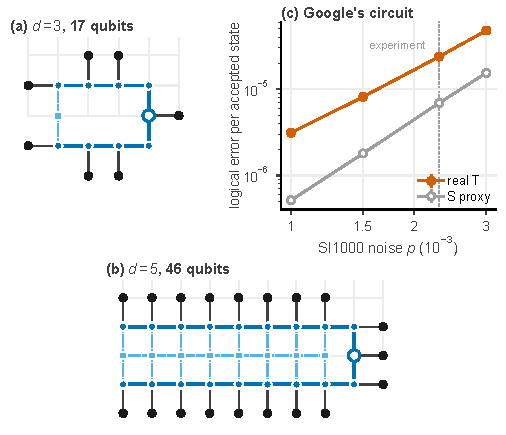
\includegraphics[width=\columnwidth]{fig_nn.pdf}
\caption{(a), (b)~Nearest-neighbour cat checks on a square grid: data qubits (black), the cat path (blue) grown from its middle (open circle), and verification ancillas (light blue) with the parities they measure (dashed). (c)~Logical error per accepted state of the circuit of Google's experiment~\cite{googlecultivation} (two checks with error-correction cycles) under SI1000 noise, with real T gates (vermillion) and with S gates (grey), at equal acceptance. The experiment ran at $p\approx2.3\times10^{-3}$ (dotted).}
\label{fig:nn}
\end{figure}

%
\section{Outlook}
Cultivation is judged by simulations that replace its T gates by S gates. Theorem~\ref{thm:main} replaces this shortcut by an exact criterion, one stabilizer code on the T gates, and Theorem~\ref{thm:gauss} makes the criterion fast enough to certify realistic circuits. The answer it gives is that the checks in use today keep only about half their distance, for a reason that Lemma~\ref{lem:completion} makes precise, and that checks built to avoid that reason keep all of it, on hardware with nearest-neighbour connectivity and at lower cost. Our results assume stochastic Pauli noise, as the simulations of cultivation do. Coherent errors and leakage, which experiments also see~\cite{googlecultivation}, are outside this model. The main open problems are a cheap way to measure stabilizers on the grid around these checks, a certificate of the full distance seven for the ladder, and lower bounds on the gates that real-T checks need (Sec.~\ref{sm:open}).

\begin{acknowledgments}
This work was carried out with the assistance of the language model Claude Opus 5.5. The final content, analysis and conclusions remain the sole responsibility of the authors. Computations used stim~\cite{stim} and Gurobi~10. This work has been supported by the European Union's HORIZON-MSCA-2023-DN-JD programme under the Horizon Europe (HORIZON) Marie Sk\l{}odowska-Curie Actions, grant agreement 101120296 (TENORS).
\end{acknowledgments}

\paragraph*{Data availability.}
The scripts, circuits and results are available at \url{https://github.com/llorebaga/Bounds_magic}. The exact evaluation of Theorem~\ref{thm:gauss} and the circuits of Propositions~\ref{prop:gsj} and~\ref{prop:vcat} are in its directory \texttt{cultivation\_exact}. The circuit chunks and state-vector data of Ref.~\cite{gsjcode} are reproduced there under the Apache License~2.0, and the circuits of Ref.~\cite{googlecultivation} are decoded from the links published with that paper.

%
\bibliography{refs,cultivation}

\clearpage
\setcounter{secnumdepth}{2}\setcounter{section}{0}\setcounter{equation}{0}\setcounter{table}{0}\setcounter{figure}{0}
\renewcommand{\thesection}{S\arabic{section}}
\renewcommand{\theequation}{S\arabic{equation}}
\renewcommand{\thetable}{S\Roman{table}}
\renewcommand{\thefigure}{S\arabic{figure}}
\onecolumngrid
\begin{center}\textbf{\large Supplemental Material}\end{center}

\section{The criterion}\label{sm:proofs}
This section states the setting precisely and proves Theorem~\ref{thm:main}, Lemma~\ref{lem:completion} and two further consequences.
\paragraph*{Circuits and protocols.}
Let $|T\rangle=(|0\rangle+\omega|1\rangle)/\sqrt2$ with $\omega=e^{i\pi/4}$. A \emph{Clifford+T protocol} acts on qubits initialized in $|0\rangle$ with Clifford gates, T and T$^\dagger$ gates, Pauli measurements, classical randomness, feedforward of any operation on earlier outcomes, postselection and discarding, and outputs $r$ qubits. Its target is a pure state $\tau$ with stabilizer nullity $\nu(\tau)=r$, that is, fixed by no Pauli operator other than the identity, as $|T\rangle$ and $|\CCZ\rangle$ are. A protocol is \emph{non-adaptive and fully postselected} if it is a fixed sequence of Clifford gates, T and T$^\dagger$ gates, projections $(I+sQ)/2$ with a Pauli $Q$ and a fixed sign $s$, and removals $\langle k|_q$ of qubits with fixed $k\in\{0,1\}$. T$^\dagger$ gates count as T gates. Such a circuit has a single Kraus operator $K$, and we call it \emph{correct} if $K|0\rangle$ is a nonzero multiple of $|\tau\rangle$.

\paragraph*{Faults.}
Every preparation, gate and measurement is a \emph{location}, except those declared ideal. Removals are ideal. A fault at a location is a Pauli operator on its support, applied immediately after a preparation or gate or immediately before a projection, or the flip of a projection's sign. Faults at different locations compose, and the \emph{fault space} $\fs$ is the $\F$-vector space of all assignments of Pauli operators and flips to locations, with the weight $\wt(F)$ of $F\in\fs$ the number of locations at which $F$ acts. Each location suffers each of its faults independently with probability $p\lambda>0$, so a run of an adaptive protocol is described by its random choices and observed outcomes $b$ together with the faults $F$ at the locations executed along $b$, and has Kraus operator $K_{b,F}$. The pair $(b,F)$ is \emph{harmless} if $K_{b,F}|0\rangle\in\mathbb C|\tau\rangle$, which includes rejection. The output error after postselection is $\epsilon=O(p^d)$ exactly when every run with $\wt(F)<d$ is harmless and some fault-free run is accepted. The largest such $d$ is the \emph{fault distance}. It depends only on which faults are possible, not on their probabilities as long as these are of order $p$, so it is the same, for example, under depolarizing noise, which applies one random Pauli operator per location.

\paragraph*{Ideal decoders.}
A protocol whose output is encoded is judged after an ideal decoder: projections onto the stabilizers of an $[[m,r,\delta]]$ code $Q$ on $m$ output qubits, followed by an ideal Clifford unencoding. We call the decoder \emph{admissible} if the fault-free state at its input lies in $Q$, so that it accepts the fault-free run with certainty. Its projections and the unencoding are ideal operations of the circuit, so the results below apply to the circuit together with its decoder. Simulations of cultivation use decoders of this kind~\cite{cultivation}. Without the condition, the decoder could carry out the T-dependent checks itself: nine noisy T states handed to an ideal decoder of the code of Proposition~\ref{prop:t9} below would already tolerate every single fault.

\paragraph*{Reduction to one run.}
\begin{proposition}\label{prop:branch}
Let a Clifford+T protocol have fault distance $d$, and let $b$ be any accepted fault-free run. The non-adaptive, fully postselected circuit formed by the operations executed along $b$, with every measurement replaced by the projection onto its outcome in $b$ and every discarded qubit removed with an outcome of nonzero amplitude, is correct and has fault distance at least $d$.
\end{proposition}
The proof (Sec.~\ref{sm:proofs}) uses only that a sum of positive operators is a multiple of a pure state exactly when each term is. Every lower bound on the qubits, gates or T gates of correct non-adaptive circuits of fault distance $d$ therefore holds for every accepted fault-free run of every protocol of fault distance $d$.

\paragraph*{The skeleton.}
In this notation, Theorem~\ref{thm:main} states in addition that $C$ has dimension $2^r$ with $\nu(\tau)=r$, that $\Pi_C|T\rangle^{\otimes t}\neq0$, and that a Clifford isometry $V$ maps $\Pi_C|T\rangle^{\otimes t}$ to a multiple of $|\tau\rangle$. A Z fault immediately before or after the $j$th T gate has $D=0$ and $E=Z_j$. With T$^\dagger=S^\dagger T$, Replacing every T gate by Eq.~\eqref{eq:gadget}, with its own ideal ancilla in $|T\rangle$, leaves a noisy Clifford circuit, the \emph{skeleton}, acting on $t$ ideal T states. Its fault-free Kraus operator is a code projection followed by a Clifford isometry, $c\,V\Pi_C$, as in Ref.~\cite{distillationpaper}. A Pauli fault anywhere in the skeleton can be pushed to the end of the circuit, where it flips the signs of the projections it anticommutes with and leaves a Pauli operator on the output. Sign flips that contradict a deterministic outcome annihilate the circuit. These are the detectors, $D(F)\neq0$. All other sign flips, and the output Pauli, are equivalent to a Pauli on the T inputs, by the Gottesman-Knill description of stabilizer circuits~\cite{aaronsongottesman}. This gives $E(F)$, and Eq.~\eqref{eq:collapse} is the condition that the perturbed T states still project onto the encoded target, or onto zero (Sec.~\ref{sm:proofs}).

The pair $(D,E)$ plays the role of the detector error model of a Clifford circuit~\cite{stim,delfossepaetznick,bombinzx}, with the logical observables replaced by the Pauli group on the T gates and the test on them by the collapse condition~\eqref{eq:collapse}, which is the one that decides distillation~\cite{distillationpaper}. Both maps are computed in polynomial time by following the Choi state of the skeleton symbolically. Only the collapse condition involves the T states (Sec.~\ref{sm:compute}).

\paragraph*{Detectors and checks.}
The entries of $D$ belong to the projections whose outcome is fixed in the skeleton. A projection whose outcome is fixed in the circuit but depends on the T inputs in the skeleton, such as a check after a layer of T gates, is not a detector in this sense. It is part of the code $C$, and it rejects a fault only through Eq.~\eqref{eq:collapse}, that is, only the components of $E(F)|T\rangle^{\otimes t}$ that leave the code. In the distance-three circuit of Ref.~\cite{cultivation}, 4 of the 20 projections are of this kind: the X measurement that reads out the logical check and three X-type stabilizers measured after the final T layer. Wan and Zapirain likewise find that 16 of its 20 detectors remain Pauli webs with T gates~\cite{wanzapirain}. With S gates the circuit is Clifford, and all 20 are detectors.

\paragraph*{Related descriptions.}
Replacing T gates by gadgets is standard in simulation~\cite{bravyigosset}. For cultivation, Surti \emph{et al.} observed that every Pauli fault reaches the end of the circuit as a Clifford error~\cite{surti}, Chan \emph{et al.} computed the acceptance and fidelity of a code state under such an error~\cite{chan}, and exact simulators follow faults through the T gates~\cite{soft,clifft,symft,wanzhong,takada,wanzapirain,syqma}. Theorem~\ref{thm:main} instead moves the non-Clifford part to the inputs, where one code, independent of the fault, judges a Pauli operator that depends linearly on the fault. The collapse condition is itself combinatorial: it compares signed weight distributions of the cosets of $S_C$ in its normalizer (Proposition~\ref{prop:enum}, Sec.~\ref{sm:codes}).

\paragraph*{Coherent faults.}
The new feature relative to distillation is that $E(F)$ may have an X part. Since $X|T\rangle=(|T\rangle+iZ|T\rangle)/\sqrt2$ and $XZ|T\rangle=-(i|T\rangle+Z|T\rangle)/\sqrt2$, a Pauli $E=X^uZ^v$ turns $|T\rangle^{\otimes t}$ into a superposition, with amplitudes of modulus $2^{-|u|/2}$, of the states $Z^{v+w}|T\rangle^{\otimes t}$ with $w$ supported on $u$.
For a Pauli operator $E$ on the T inputs, let $|E|_S$ be the least number of qubits on which an element of $E\langle iI,S_C\rangle$ acts.
\begin{lemma}\label{lem:shadow}
(i)~If every pattern $v+w$ with $\operatorname{supp}w\subseteq\operatorname{supp}u$ satisfies the distillation condition $\Pi_CZ^{v+w}|T\rangle^{\otimes t}\in\mathbb C\,\Pi_C|T\rangle^{\otimes t}$, then so does $X^uZ^v$, and every $F$ with $E(F)=X^uZ^v$ is harmless. (ii)~If every Z pattern of weight below $d$ satisfies it, then so does every Pauli operator $E$ with $|E|_S<d$, and $C$ has distance at least $d$.
\end{lemma}
The smallest instance of~(i) is a single check (Fig.~\ref{fig:small}a): a projection onto $|T\rangle$ rejects $Z|T\rangle$ and returns $X|T\rangle$ and $Y|T\rangle$ to $|T\rangle$ half of the time, so X and Y faults before it are harmless although they are neither detected nor stabilizers (Sec.~\ref{sm:example}). The converse of~(i) can fail, because harmful components may cancel. Part~(ii) is where cultivation and distillation meet: a code that tolerates Z faults on fewer than $d$ inputs tolerates every Pauli fault on them, and, since no Pauli operator fixes the target, it has no logical operator of weight below $d$.

\begin{proof}[Proof of Proposition~\ref{prop:branch}]
For a fixed fault configuration, the unnormalized accepted output of the protocol is $\sum_{b'}q\,K_{b',F'}\rho_0K_{b',F'}^\dagger$, summed over accepted runs $b'$ and the faults $F'$ along them, with probabilities $q>0$. This is exact for stochastic Pauli noise, because faults are sampled classically at the locations actually executed. A run $(b,F)$ is harmless exactly when its own term is a multiple of $|\tau\rangle\langle\tau|$. Fix an accepted fault-free run $b$. Along $b$, every random choice and every measurement outcome is fixed, so the operations executed along $b$ form a non-adaptive circuit, and for every fault configuration $F$ at its locations, $K_{b,F}$ is the Kraus operator of this circuit with $F$ inserted, postselected on the outcomes of $b$. A discarded qubit contributes a partial trace, $\sum_k\langle k|\cdot|k\rangle$. If the sum is a multiple of a pure state, each term is, so replacing the partial trace by the removal $\langle k|$ for an outcome $k$ with $\langle k|K_{b,\emptyset}|0\rangle\neq0$ keeps the circuit correct and every harmless configuration harmless. Hence every configuration with $\wt(F)<d$ is harmless in the circuit. The removals are ideal and add no locations.
\end{proof}

\begin{proof}[Proof of Theorem~\ref{thm:main}]
\emph{Skeleton.} Eq.~\eqref{eq:gadget} follows from $\mathrm{CX}_{q\to a}(\alpha|0\rangle+\beta|1\rangle)(|0\rangle+\omega|1\rangle)/\sqrt2$, whose component with $a$ in $|0\rangle$ is $(\alpha|0\rangle+\beta\omega|1\rangle)/\sqrt2$. Introduce one ancilla $a_j$ per T gate, prepared ideally in $|T\rangle$, and write T$^\dagger=S^\dagger T$ with an ideal $S^\dagger$. A fault of the $j$th T gate acts after the gadget. The circuit becomes $K_F=2^{t/2}K_{S,F}(|0\rangle\otimes|T\rangle^{\otimes t})$, where the skeleton $K_{S,F}$ consists of Clifford gates, projections and removals, and $F$ is inserted at the same qubits and times. Let $M_F=K_{S,F}(|0\rangle\otimes\cdot)$, a linear map from $t$ qubits to $r$ qubits, and $M=M_0$. As in the proof of Theorem~1 of Ref.~\cite{distillationpaper}, $M$ applied to half of $t$ Bell pairs gives a stabilizer state on $t+r$ qubits, and by the local-Clifford normal form of bipartite stabilizer states $M=c\,V\Pi_C$ with a stabilizer code $C$ on $t$ qubits and a Clifford isometry $V$ from $C$ onto its range. The range contains $|\tau\rangle$ and is a stabilizer subspace. Since no Pauli operator other than the identity fixes $\tau$, it is the whole output space, so $\dim C=2^r$ and $V$ is unitary from $C$ onto $(\mathbb C^2)^{\otimes r}$.

\emph{Signs.} Treat each removal $\langle k|_q$ as a projection of $Z_q$ with sign $(-1)^k$ followed by an ideal removal, and let $\sigma\in\F^\mu$ list the signs of all $\mu$ projections relative to the circuit, so that $M^{(0)}=M$. Let $|\Psi^{(\sigma)}\rangle=(M^{(\sigma)}\otimes I)\sum_x|x\rangle|x\rangle$ be the unnormalized Choi vector. Following the circuit with the stabilizer formalism~\cite{aaronsongottesman}, the Choi vector stays a pure stabilizer state, so the Pauli of every projection either anticommutes with a current stabilizer or is one up to sign. In the first case the projection halves the squared norm and replaces that stabilizer by the projected Pauli with the chosen sign, and in the second it keeps the state or annihilates it, depending on the sign. The unsigned stabilizer groups and the norms of the nonzero $|\Psi^{(\sigma)}\rangle$ are therefore independent of $\sigma$. The signs required by the deterministic projections are affine functions of the earlier signs, so $|\Psi^{(\sigma)}\rangle\neq0$ exactly when $D_0\sigma=0$ for a linear map $D_0$. Two stabilizer states with the same unsigned group and norm differ by a Pauli operator and a phase, and the Pauli is determined by the sign difference modulo the stabilizer group, linearly. Hence, for $D_0\sigma=0$, $|\Psi^{(\sigma)}\rangle=\zeta_\sigma(A_\sigma\otimes B_\sigma)|\Psi^{(0)}\rangle$ with $|\zeta_\sigma|=1$ and Paulis $A_\sigma$ on the output and $B_\sigma$ on the reference, that is, $M^{(\sigma)}=\zeta_\sigma A_\sigma MB_\sigma^{\mathsf T}$.

\emph{Faults.} A Pauli $P$ inserted after an operation is moved to the end of the circuit: a Clifford gate $G$ turns it into $GPG^\dagger$, and a projection $(I+sQ)$ with which it anticommutes becomes $(I-sQ)$ as $P$ passes it. A removal absorbs the Z part of $P$ on the removed qubit, and its projection turns the X part into a sign flip. A sign flip changes $\sigma$ directly. Hence $M_F=\zeta\,P_{\mathrm{out}}(F)\,M^{(s(F))}$ with a phase $\zeta$, a Pauli $P_{\mathrm{out}}(F)$ on the output and a sign vector $s(F)$, both linear in $F$. Set $D(F)=D_0s(F)$, where $D_0$ has one row per projection, nonzero only for the projections whose outcome is fixed in the skeleton. If $D(F)\neq0$, then $M_F=0$ and the configuration is rejected. Otherwise $M_F=\zeta'P_{\mathrm{out}}A_{s}MB_{s}^{\mathsf T}$. For an output Pauli $R$, write $V\Pi_C=W(I\otimes\langle0|^{\otimes(t-r)})U\Pi_C$ with Clifford unitaries $U$ on $t$ qubits, mapping $C$ onto $(\mathbb C^2)^{\otimes r}\otimes|0\rangle^{\otimes(t-r)}$, and $W$ on $r$ qubits. Then $RM=ML$ with the Pauli $L=U^\dagger(W^\dagger RW\otimes I)U$, which commutes with the stabilizers of $C$. Hence $M_F=\zeta''M\,E(F)$ with $E(F)=L(P_{\mathrm{out}}A_s)B_s^{\mathsf T}$. Finally, $ME\propto ME'$ holds exactly when $E'E^\dagger$ acts on $C$ as a scalar, that is, lies in $\langle iI,S_C\rangle$, because $V$ is injective on $C$ and a Pauli that anticommutes with a stabilizer maps $C$ to an orthogonal code. So $E$ is well defined and linear modulo $\langle iI,S_C\rangle$.

\emph{Collapse.} $K_F|0\rangle=2^{t/2}\zeta''c\,V\Pi_CE(F)|T\rangle^{\otimes t}$ and $K_0|0\rangle\propto V\Pi_C|T\rangle^{\otimes t}\propto|\tau\rangle$. Since $V$ is injective on $C$, $K_F|0\rangle\in\mathbb C|\tau\rangle$ exactly when Eq.~\eqref{eq:collapse} holds.

\emph{Z faults at T gates.} A Z fault after the gadget of the $j$th T gate on qubit $q$ satisfies $Z_q\langle0|_a\mathrm{CX}_{q\to a}=\langle0|_aZ_aZ_q\mathrm{CX}_{q\to a}=\langle0|_a\mathrm{CX}_{q\to a}Z_a$, using $\langle0|_a=\langle0|_aZ_a$ and $\mathrm{CX}_{q\to a}Z_a=Z_qZ_a\mathrm{CX}_{q\to a}$. It acts as $Z$ on the ideal input $a_j$, so $D=0$ and $E=Z_j$. A Z fault before the gate is the same, because Z commutes with T and with $S^\dagger$.
\end{proof}

\begin{proof}[Proof of Lemma~\ref{lem:shadow}]
(i)~On one qubit, $X|T\rangle=(|T\rangle+iZ|T\rangle)/\sqrt2$, $XZ|T\rangle=-(i|T\rangle+Z|T\rangle)/\sqrt2$ and $Y=iXZ$, so up to a phase $X^uZ^v|T\rangle^{\otimes t}=\sum_w\gamma_wZ^{v+w}|T\rangle^{\otimes t}$, summed over $w$ with $\operatorname{supp}w\subseteq\operatorname{supp}u$ and with $|\gamma_w|=2^{-|u|/2}$. If each projected term lies on the line $\mathbb C\,\Pi_C|T\rangle^{\otimes t}$, so does their sum, and Theorem~\ref{thm:main} applies. (ii)~Multiplying $E$ by an element of $\langle iI,S_C\rangle$ changes $\Pi_CE|T\rangle^{\otimes t}$ only by a phase, so we may take $E=X^uZ^v$ acting on fewer than $d$ qubits. Every pattern $v+w$ in~(i) is supported on these qubits and so has weight below $d$, and~(i) applies. Now let $E$ commute with $S_C$ and $|E|_S<d$. Then $E$ commutes with $\Pi_C$, and $E\Pi_C|T\rangle^{\otimes t}=\Pi_CE|T\rangle^{\otimes t}$ is a multiple of $\Pi_C|T\rangle^{\otimes t}$, nonzero because $E$ is unitary. Through the isometry $V$, $E$ acts on $C$ as a Pauli operator $P$ on $r$ qubits up to a phase, and $|\tau\rangle$ is an eigenvector of $P$. A Hermitian multiple $P'$ of $P$ has eigenvalues $\pm1$, so $P'$ or $-P'$ fixes $|\tau\rangle$. Since $\nu(\tau)=r$, $P'=\pm I$. Hence $E$ acts on $C$ as a scalar, that is, $E\in\langle iI,S_C\rangle$, and every logical operator outside $\langle iI,S_C\rangle$ acts on at least $d$ qubits.
\end{proof}

\begin{proof}[Proof of Lemma~\ref{lem:completion}]
For $U_q=T^{\pm1}$, $U_qXU_q^\dagger=\bar\omega^{\pm1}S^{\pm1}X$ and $S^{\pm1}=\omega^{\pm1}(I\mp iZ)/\sqrt2$. The error immediately after the layer is therefore, up to a phase, $\prod_{q\in u}(I\mp iZ_q)X^u/2^{|u|/2}=2^{-|u|/2}\sum_{w\subseteq u}c_wZ^wX^u$ with $c_w=\prod_{q\in w}(\mp i)$. The faults after the layer give $X^{\ell\setminus u}Z^wX^u=\pm Z^wX^\ell$. The ideal decoder projects onto the reference syndrome. $X^\ell$ is a logical operator, so it commutes with all stabilizers. $Z^w$ with $w\subseteq u\subsetneq\ell$ has $|w|<\delta$, so it is not a nontrivial logical operator and commutes with all X stabilizers only if it is a Z stabilizer, which by assumption happens only for $w=\emptyset$. Every other component is mapped by the projection to an orthogonal syndrome space and removed. The accepted component is $2^{-|u|/2}X^\ell$ applied to the fault-free state, of relative probability $2^{-|u|}$, and it decodes to $X_L|\tau\rangle$. For $|\tau\rangle=|T\rangle$, $|\langle T|X|T\rangle|^2=1/2$, so the output is wrong with probability $1/2$. With Y in place of the last X, the output is $X_LZ_L|\tau\rangle$ up to a phase, orthogonal to $|T\rangle$. In the proxy, $SXS^\dagger=Y$ up to a phase, so the error after the layer is the Pauli $Z^uX^\ell$ up to a phase. $Z^u$ with $\emptyset\neq u\subsetneq\ell$ is neither a stabilizer nor a logical operator, so it has a nontrivial syndrome and the configuration is rejected.
\end{proof}

\paragraph*{Two further consequences.}
The complement symmetry of distillation~\cite{distillationpaper} and the code distance of an ideal decoder give the following two statements. Neither is needed in the main text.
\begin{corollary}\label{cor:galois}
If all Pauli expectations of $\tau$ are rational, a fault configuration $F$ of a correct non-adaptive circuit is harmless if and only if $F+Z_{\mathcal T}$ is, where $Z_{\mathcal T}$ places a Z fault after every T gate.
\end{corollary}
\begin{proof}
The automorphism $\sigma$ of $\mathbb Q(\sqrt2,i)$ that flips the sign of $\sqrt2$ and fixes $i$ maps $\omega$ to $-\omega$, so, applied entrywise, it maps T and T$^\dagger$ to $ZT$ and $ZT^\dagger$. It maps every Clifford gate to itself up to a global phase, because up to such a phase the entries of a Clifford gate are $2^{-k/2}$ times Gaussian integers, and it fixes projections, Pauli faults and $|0\rangle$. Hence $\sigma$ maps $K_F|0\rangle\langle0|K_F^\dagger$ to $K_{F+Z_{\mathcal T}}|0\rangle\langle0|K_{F+Z_{\mathcal T}}^\dagger$, as $\sigma$ commutes with complex conjugation. It fixes $|\tau\rangle\langle\tau|$, whose entries lie in $\mathbb Q(i)$ because its Pauli coefficients are rational. Since $\sigma^2$ is the identity, one of the two operators is a multiple of $|\tau\rangle\langle\tau|$ exactly when the other is.
\end{proof}
\begin{proposition}\label{prop:singleton}
If a correct circuit ends with an admissible ideal decoder for an $[[m,r,\delta]]$ code, and each of the $m$ qubits has an idle location immediately before the decoder, then its fault distance $d$ is at most $\delta$, and $m\geq r+2(d-1)$.
\end{proposition}
\begin{proof}
A logical Pauli of weight $\delta$ placed at the idle locations commutes with the stabilizers, passes the decoder and applies a nontrivial Pauli to the decoded state, which differs from $|\tau\rangle$ because $\nu(\tau)=r$. The inequality is the quantum Singleton bound~\cite{knilllaflamme}.
\end{proof}

\section{Deterministic checks and Gauss sums}\label{sm:gauss}
Lemma~\ref{lem:shadow}(i) decides harmlessness when every component collapses. In cultivation, the components behave as on a stabilizer code, and the collapse condition can be decided exactly, without enumerating the cosets of $S_C$ as in Proposition~\ref{prop:enum}.
\begin{definition}\label{def:dc}
A correct circuit for $|T\rangle$ has \emph{deterministic checks} if there are a subspace $\Sigma\subseteq\F^t$ and $\ell\in\F^t$ such that $Z^e\in\pm S_C$ for $e\in\Sigma$, $Z^\ell$ commutes with $S_C$ and $VZ^\ell V^\dagger$ acts on the output as $Z$, and $\Pi_CZ^e|T\rangle^{\otimes t}=0$ for every $e\notin\Sigma\cup(\ell+\Sigma)$.
\end{definition}
Every Z error on the T gates is then a stabilizer of $C$, the logical Z, or rejected with certainty. This is the case when every check measures an operator of which the target is an eigenstate, and not for code-based distillation, where Z errors on the inputs are detected only with some probability. The signs $Z^e=\sigma(e)g_e$, $g_e\in S_C$, define a character $\sigma$ of $\Sigma$, which we extend to a character $\chi$ of $\F^t$.
\begin{theorem}\label{thm:gaussfull}
For a circuit with deterministic checks and a configuration with $D(F)=0$ and $E(F)=X^aZ^b$,
\begin{equation}
 \Pi_CE(F)|T\rangle^{\otimes t}=\mu\,2^{-|a|/2}\bigl(g_0+g_1Z^\ell\bigr)\Pi_C|T\rangle^{\otimes t},
 \label{eq:out}
\end{equation}
with $|\mu|=1$ and, for $c\in\{0,1\}$,
\begin{equation}
 g_c=\sum_{w\leq a,\;w+b\in c\ell+\Sigma}i^{|w|}\,\chi(w+b+c\ell).
 \label{eq:g}
\end{equation}
The configuration is accepted with probability $2^{-|a|}(|g_0|^2+|g_1|^2)$ relative to the fault-free run, its wrong output has weight $2^{-|a|}|g_1|^2$, and it is harmful if and only if $g_1\neq0$.
\end{theorem}
Theorem~\ref{thm:gauss} of the main text restates this, with $a$ the X part of $E(F)$ and Proposition~\ref{prop:poly} below for the cost.
Definition~\ref{def:dc} removes every Z pattern outside the two cosets, and the two surviving terms are orthogonal and of equal norm because $\langle T|Z|T\rangle=0$ (Sec.~\ref{sm:proofs}). The sums~\eqref{eq:g} run over affine subspaces $w_0+\langle k_1,\dots,k_m\rangle$ of $\F^{|a|}$, and by inclusion and exclusion $|w_0+\sum_lz_lk_l|\equiv|w_0|+\sum_lz_l(|k_l|-2|w_0\wedge k_l|)-2\sum_{l<m}z_lz_m|k_l\wedge k_m|\pmod4$, so each $g_c$ is an exponential sum $\sum_{z\in\F^m}i^{q(z)}$ of a $\Z_4$-valued quadratic form.
\begin{proposition}\label{prop:poly}
Each $g_c$ is computed with $O(t^3)$ operations, and $|g_c|$ is zero or a power of $\sqrt2$. In particular the acceptance and the bad weight of every fault configuration are dyadic rationals.
\end{proposition}
Summing out one variable of $q$ multiplies the sum by $1\pm i$ and adds a parity to $q$, or multiplies it by two and eliminates a second variable through a linear constraint, or shows that it vanishes (Sec.~\ref{sm:proofs}). The coherence of real T gates enters only through these sums. Treating the terms of Eq.~\eqref{eq:g} one at a time, and calling a configuration harmful when one of them lies in $\ell+\Sigma$, gives a lower bound on the fault distance that equals one for every circuit we studied: a single X fault before a check has such a term, which the check removes only through the cancellation $g_1=0$.

\begin{proof}[Proof of Theorem~\ref{thm:gaussfull}]
On one qubit, $|T\rangle=(|0\rangle+\omega|1\rangle)/\sqrt2$, $Z|T\rangle=(|0\rangle-\omega|1\rangle)/\sqrt2$ and $X|T\rangle=\omega(|0\rangle+\bar\omega|1\rangle)/\sqrt2$. Writing $|0\rangle+\bar\omega|1\rangle=\alpha(|0\rangle+\omega|1\rangle)+\beta(|0\rangle-\omega|1\rangle)$ gives $\alpha+\beta=1$ and $\alpha-\beta=\bar\omega^2=-i$, so $\alpha=\bar\omega/\sqrt2$, $\beta=i\bar\omega/\sqrt2$ and $X|T\rangle=(|T\rangle+iZ|T\rangle)/\sqrt2$. Taking the tensor product over $\mathrm{supp}\,a$ and using $X^aZ^b=(-1)^{|a\wedge b|}Z^bX^a$,
\begin{equation}
 X^aZ^b|T\rangle^{\otimes t}=(-1)^{|a\wedge b|}\,2^{-|a|/2}\sum_{w\leq a}i^{|w|}Z^{b+w}|T\rangle^{\otimes t}.
\end{equation}
Apply $\Pi_C$. By Definition~\ref{def:dc}, the terms with $b+w\notin\Sigma\cup(\ell+\Sigma)$ vanish. If $e\in c\ell+\Sigma$, then $e+c\ell\in\Sigma$ and $Z^{e+c\ell}=\sigma(e+c\ell)g$ with $g\in S_C$, and $\Pi_Cg=\Pi_C$. Since $Z^\ell$ commutes with $S_C$, it commutes with $\Pi_C$, so $\Pi_CZ^e|T\rangle^{\otimes t}=\chi(e+c\ell)Z^{c\ell}\Pi_C|T\rangle^{\otimes t}$. This proves Eq.~\eqref{eq:out} with $\mu=(-1)^{|a\wedge b|}$. The vector $Z^\ell\Pi_C|T\rangle^{\otimes t}$ has the same norm as $\Pi_C|T\rangle^{\otimes t}$, and $V$ maps the two to multiples, of equal modulus, of $Z|T\rangle$ and $|T\rangle$, which are orthogonal. The acceptance and the bad weight follow, and the bad weight is positive exactly when $g_1\neq0$.
\end{proof}

\begin{proof}[Proof of Proposition~\ref{prop:poly}]
The set $\{w\leq a: w+b\in c\ell+\Sigma\}$ is empty or an affine subspace $w_0+\langle k_1,\dots,k_m\rangle$ of $\F^{|a|}$, found by Gaussian elimination in $O(t^3)$. For binary vectors $v_0,\dots,v_m$, inclusion and exclusion give $|v_0+\dots+v_m|=\sum_{S\neq\emptyset}(-2)^{|S|-1}|\bigwedge_{s\in S}v_s|$, and the terms with $|S|\geq3$ vanish modulo four. With $\chi(w)=(-1)^{x\cdot w}$ and $2(x\cdot w)\bmod4$ linear in $z$, the summand of Eq.~\eqref{eq:g} is $i^{q(z)}$ with
\begin{equation}
 q(z)=q_0+\sum_lL_lz_l+2\sum_{l<m}B_{lm}z_lz_m,\quad L_l=|k_l|-2|w_0\wedge k_l|+2\,x\cdot k_l,\quad B_{lm}=|k_l\wedge k_m|\bmod2 .
\end{equation}
To sum out $z_v$, let $N$ be the set of its neighbours ($B_{vm}=1$) and $y=\bigoplus_{m\in N}z_m$. The sum over $z_v$ is $1+i^{L_v}(-1)^y$. If $L_v$ is odd, this is $(1+i)\,i^{3y}$ or $(1-i)\,i^{y}$. The parity $y$, read as an integer modulo four, is $\sum_mz_m-2\sum_{m<m'}z_mz_{m'}$, so $q$ stays quadratic. If $L_v$ is even, it is $2[y=L_v/2]$: if $N$ is empty, the sum vanishes or is multiplied by two. Otherwise the constraint expresses one variable of $N$ as a parity of the others, which is substituted into $q$ in the same way. Each step costs $O(m^2)$ and multiplies the modulus by $\sqrt2$ or $2$, or returns zero, so $|g_c|$ is zero or a power of $\sqrt2$, and the acceptance $2^{-|a|}(|g_0|^2+|g_1|^2)$ and bad weight $2^{-|a|}|g_1|^2$ are dyadic. We checked the procedure against direct summation on 400 random forms with up to eight variables.
\end{proof}

\section{Cultivation as distillation}\label{sm:distill}
This section proves Theorem~\ref{cor:exact}. Its first half, that a circuit of fault distance $d$ needs as many T gates as an order-$d$ distillation protocol needs inputs, follows from Theorem~\ref{thm:main} directly. Its second half, that this number of T gates also suffices, needs a construction.
\begin{corollary}\label{cor:tcount}
In a noise model in which every T gate may suffer a Z fault, every accepted run of a protocol of fault distance $d$ executes at least $n_{\min}(\tau,d)$ T gates, the least number of noisy T inputs of any order-$d$ distillation protocol for $\tau$.
\end{corollary}
\begin{proof}
By Proposition~\ref{prop:branch} it suffices to consider a correct non-adaptive circuit with $t$ T gates and fault distance $d$. Configurations of Z faults at T gates have $D=0$ and $E=Z^e$, so by Theorem~\ref{thm:main} each with $|e|<d$ satisfies $\Pi_CZ^e|T\rangle^{\otimes t}\in\mathbb C\,\Pi_C|T\rangle^{\otimes t}$. Measuring the stabilizers of $C$ on $t$ noisy T states, postselecting and decoding with $V$ is therefore an order-$d$ distillation protocol~\cite{distillationpaper}.
\end{proof}
The proof uses only the \emph{order} $d_C$ of the code, the least weight of a Z pattern that violates the distillation condition, which is the suppression order of the distillation protocol that measures $C$ on noisy T states. The Clifford part limits the fault distance in a second way, by spreading faults. We call $d_{\mathrm{sp}}=\min\{\wt(F):D(F)=0,\ |E(F)|_S>\wt(F)\}$, the least number of undetected faults whose Pauli operator on the T inputs is heavier than their number, the \emph{spreading distance} of the circuit.
\begin{theorem}\label{thm:attain}
A correct non-adaptive circuit with code $C$ has fault distance $d$ with $\min(d_C,d_{\mathrm{sp}})\leq d\leq d_C$. Conversely, for every stabilizer code $C$ on $t$ qubits that encodes a target as $\Pi_C|T\rangle^{\otimes t}\neq0$, there is a correct non-adaptive circuit with $t$ T gates and an admissible ideal decoder whose code is $C$ and whose fault distance is $d_C$.
\end{theorem}
The upper bound is the proof of Corollary~\ref{cor:tcount}, and the lower bound is Lemma~\ref{lem:shadow}(ii). For the converse (Sec.~\ref{sm:proofs}), the circuit applies T to $t$ qubits in $|{+}\rangle$, so that its T inputs are its data, and measures the generators of $C$ one after another with cat states~\cite{shor}, each checked by $d_C-1$ rounds of parity measurements. A cat state that passes a fault-free round has no X error, so $k$ faults in one measurement leave a data error of weight at most $k$. The output stays encoded in $C$, and the ideal decoder, which measures $C$ again, rejects every run whose recorded signs disagree with the data error. Hence $d_{\mathrm{sp}}\geq d_C$.

The equality combines Corollary~\ref{cor:tcount} with Theorem~\ref{thm:attain} for the code of an optimal distillation protocol, which has distance at least $d$ by Lemma~\ref{lem:shadow}(ii). The last bounds follow from Rains' theorem that a quantum code of length $n$ corrects at most $\lfloor(n+1)/6\rfloor$ errors~\cite{rains}. The exact values of Ref.~\cite{distillationpaper} thus hold for cultivation: fault distance two needs nine T gates for one T state and eight for $|\CCZ\rangle$. The distance bound is new for distillation too. The linear-programming bound for stabilizer codes with Rains' shadow enumerator~\cite{shorlaflamme,rains}, certified in exact arithmetic (Table~\ref{tab:lp}), raises the lower bounds for one T state at $d=6,\dots,12$ from $\max(2d,d+7)$ to $16$, $17$, $22$, $23$, $28$, $29$ and $34$, and for $|\CCZ\rangle$ at $d=4,\dots,8$ from $11$, $12$, $13$, $15$ and $17$ to $12$, $14$, $17$, $20$ and $23$.

\begin{lemma}[Checked cat-state measurement]\label{lem:cat}
Let a Pauli operator $g$ act on $w$ data qubits with letters $P_1,\dots,P_w$. Prepare $(|0\rangle^{\otimes w}+|1\rangle^{\otimes w})/\sqrt2$ on cat qubits $c_1,\dots,c_w$ by preparing $c_1$ in $|{+}\rangle$ and the others in $|0\rangle$ and applying CNOTs from $c_1$. In each of $\ell$ rounds, measure $Z_{c_1}Z_{c_i}$ for $i=2,\dots,w$ with a fresh ancilla in $|0\rangle$, the target of CNOTs from $c_1$ and $c_i$, and keep the outcome $+1$. Apply controlled-$P_i$ from $c_i$ to the $i$th data qubit for every $i$. Measure every $c_i$ in the X basis and keep the runs whose outcomes have product $s$. If at most $\ell$ faults occur in this gadget and the run is kept, it acts on the data as $R\,(I+s'g)/2$ up to a nonzero scalar, with $s'=\pm s$ and a Pauli operator $R$ for which $R$ or $Rg$ acts on at most as many qubits as there are faults.
\end{lemma}
\begin{proof}
Without faults, X outcomes with product $(-1)^{|x|}$ leave a nonzero multiple of $[I+(-1)^{|x|}g]/2$ on the data. Push every fault to the end of the gadget. Z errors on cat qubits, which Z errors on the ancillas also produce, and flips of the X measurements change the product of the X outcomes. X errors on the ancillas and flips of their measurements change only the checks. A Pauli on a data qubit before its controlled Pauli can be moved after it, at the cost of a Z error on its cat qubit when it anticommutes with $P_i$. Let $x\in\F^w$ mark the X errors on the cat qubits at the controlled Paulis. They reach the data as $P^x=\bigotimes_iP_i^{x_i}$, and $P^{x+\mathbf1}=\pm gP^x$. During the rounds the cat qubits are only controls of CNOTs, so a fault there changes at most one entry of $x$, as does a fault on a cat qubit before its own controlled Pauli, and a fault in a controlled Pauli or on a data qubit adds a Pauli on one data qubit, since an X error on $c_i$ after its controlled Pauli no longer spreads. If the preparation of the cat state is fault-free, $x$ starts at $\mathbf0$. Otherwise at most $\ell-1$ faults fall into the $\ell$ rounds, so one round is fault-free. It reads $x_1+x_i$ correctly for every $i$, so a kept run has $x\in\{\mathbf0,\mathbf1\}$ after it, and only later faults change $x$. In both cases the data error is $R$ or $\pm Rg$ with $R$ acting on at most as many qubits as there are faults.
\end{proof}

\begin{proof}[Proof of Theorem~\ref{thm:attain}]
\emph{Bounds.} Choose a pattern $e$ of weight $d_C$ that violates the distillation condition. Z faults at the corresponding T gates have $D=0$ and $E=Z^e$ (Theorem~\ref{thm:main}), so they are harmful, and $d\leq d_C$. If $\wt(F)<\min(d_C,d_{\mathrm{sp}})$ and $D(F)=0$, then $|E(F)|_S\leq\wt(F)<d_C$, and $F$ is harmless by Lemma~\ref{lem:shadow}(ii).

\emph{Construction.} Let $g_1,\dots,g_m$ generate $S_C$, with signs $s_k$. The circuit prepares $t$ data qubits in $|{+}\rangle$, applies T to each, measures $g_1,\dots,g_m$ in turn with the gadget of Lemma~\ref{lem:cat}, with $\ell=d_C-1$ and $s=s_k$, and passes the data to the ideal decoder of $C$, which projects onto $(I+s_kg_k)/2$ for every $k$ and unencodes. Without faults the checks of the cat states are deterministic and the measurements apply $\Pi_C$, so the output is a nonzero multiple of $\Pi_C|T\rangle^{\otimes t}$, the circuit is correct, and the decoder is admissible. In the skeleton, the gadget of a T gate on $|{+}\rangle$ maps its input to the data qubit identically, $\sqrt2\langle0|_a\mathrm{CX}_{q\to a}|{+}\rangle_q|\psi\rangle_a=|\psi\rangle_q$, so the code of the circuit is $C$. Let $F$ have fewer than $d_C$ faults, and let every check of the cat states pass. By Lemma~\ref{lem:cat} the $k$th measurement acts as $R_k(I+s'_kg_k)/2$, with $R_k$ or $R_kg_k$ acting on at most as many qubits as there are faults in that gadget, and every other fault, on a T gate or an idle data qubit, is a Pauli operator on one data qubit. So is a fault on the preparation of $|{+}\rangle$, which leaves $|{+}\rangle$ or $|{-}\rangle$, with $T|{-}\rangle=ZT|{+}\rangle$. Move all these Paulis to the T inputs. A Pauli $R$ moved past $(I+s'g)/2$ turns it into $(I+(-1)^{\langle R,g\rangle}s'g)/2$, so the circuit applies $\prod_k(I+s_kg_k)/2\cdot\prod_k(I+s''_kg_k)/2\cdot R\,|T\rangle^{\otimes t}$ with signs $s''_k$, where $R$ is the product of all the Paulis. Since the projections commute, this vanishes unless $s''_k=s_k$ for every $k$, and it is then a multiple of $\Pi_CR|T\rangle^{\otimes t}$. Replacing $R_k$ by $R_kg_k$ changes $R$ only within $R\langle iI,S_C\rangle$, so $|R|_S\leq\wt(F)<d_C$, and Lemma~\ref{lem:shadow}(ii) shows that $F$ is harmless. Faults that fail a check are rejected. Hence the fault distance is at least $d_C$, and by the bound above it equals $d_C$.
\end{proof}

\begin{proof}[Proof of Theorem~\ref{cor:exact}]
By Corollary~\ref{cor:tcount}, every accepted run executes at least $n_{\min}(\tau,d)$ T gates. By Theorem~1 of Ref.~\cite{distillationpaper}, an order-$d$ distillation protocol on $n=n_{\min}(\tau,d)$ inputs yields a stabilizer code $C$ on $n$ qubits whose projection of $|T\rangle^{\otimes n}$ encodes $\tau$ and satisfies the distillation condition for all patterns of weight below $d$, so $d_C\geq d$. Theorem~\ref{thm:attain} turns $C$ into a circuit with $n$ T gates and fault distance $d_C\geq d$. By Lemma~\ref{lem:shadow}(ii), $C$, and the code of every order-$d$ distillation protocol, has $r$ logical qubits and distance at least $d$. Such a code corrects $\lfloor(d-1)/2\rfloor$ errors, and by Ref.~\cite{rains} its length is at least $6\lfloor(d-1)/2\rfloor-1$, which is $3d-4$ for odd $d$. For even $d$, feeding one input of an order-$d$ protocol with $I/2$ gives an order-$(d-1)$ protocol~\cite{distillationpaper}, so $n_{\min}(\tau,d)\geq n_{\min}(\tau,d-1)+1\geq3d-6$.
\end{proof}

\section{Codes on the T gates}\label{sm:codes}
\paragraph*{A combinatorial form of the collapse condition.}
For a Hermitian Pauli operator $P$ on $t$ qubits, $\langle T|^{\otimes t}P|T\rangle^{\otimes t}$ is $\pm2^{-\wt(P)/2}$ if $P$ contains no Z, with the sign of $P$ as a product of the letters I, X and Y, and zero otherwise, because $\langle T|X|T\rangle=\langle T|Y|T\rangle=1/\sqrt2$ and $\langle T|Z|T\rangle=0$.
\begin{proposition}\label{prop:enum}
For a Pauli operator $E$ on the T inputs and a Hermitian Pauli operator $L$ that commutes with $S_C$, let
\begin{equation}
 A_E(L)=\sum_{g\in S_C}(-1)^{\langle E,Lg\rangle}\,\langle T|^{\otimes t}Lg|T\rangle^{\otimes t},
 \label{eq:enum}
\end{equation}
the signed count of the elements of $LS_C$ without Z, weighted by $2^{-\wt/2}$ and by their commutation with $E$. Then $E$ satisfies Eq.~\eqref{eq:collapse} if and only if $A_E(L)A_0(I)=A_E(I)A_0(L)$ for every such $L$. It suffices to take one $L$ from each of the $4^r$ cosets of $\langle iI,S_C\rangle$ in the normalizer of $S_C$.
\end{proposition}
\begin{proof}
Let $\psi_E=\Pi_CE|T\rangle^{\otimes t}$, with $\Pi_C=2^{r-t}\sum_{g\in S_C}g$. Since $L$ commutes with $\Pi_C$ and $E^\dagger LgE=(-1)^{\langle E,Lg\rangle}Lg$, we have $\langle\psi_E|L|\psi_E\rangle=\langle T|^{\otimes t}E^\dagger L\Pi_CE|T\rangle^{\otimes t}=2^{r-t}A_E(L)$. The operators $\Pi_CL\Pi_C$ span the operators on $C$, so the rank-one operators $|\psi_E\rangle\langle\psi_E|$ and $|\psi_0\rangle\langle\psi_0|$ are proportional, with ratio $A_E(I)/A_0(I)\geq0$, exactly when the identities hold, and $\psi_E\in\mathbb C\,\psi_0$ exactly when they are proportional, including $\psi_E=0$. Replacing $L$ by $Lg$ with $g\in S_C$ does not change $A_E(L)$.
\end{proof}
Each $A_E(L)$ has the form $a+b\sqrt2$ with dyadic rationals $a$ and $b$, so each identity is a pair of identities between rationals. For $E=Z^e$ the sums are the signed weight enumerators with which Rall described distillation~\cite{rall}. The test needs $4^r$ sums over the $2^{t-r}$ elements of $S_C$, in place of state vectors of dimension $2^t$. We compared it with state vectors for all $7168$ Pauli operators on $25$ random codes with $t\leq5$ and $r\leq2$, without a disagreement.

\paragraph*{Linear-programming bound.}
For an $[[n,k]]$ stabilizer code with stabilizer group $S$, let $A_j$ and $B_j$ be the numbers of elements of weight $j$ of $S$ and of its normalizer, up to phases, and let $S_j$ be the number of Pauli operators of weight $j$ in its shadow, which commute with the elements of even weight of $S$ and anticommute with those of odd weight. These numbers satisfy~\cite{shorlaflamme,rains}
\begin{align*}
&A_0=1,\qquad\textstyle\sum_jA_j=2^{n-k},\qquad B_j=2^{k-n}\sum_iK_j(i)A_i,\qquad S_j=2^{k-n}\sum_i(-1)^iK_j(i)A_i,\\
&B_j\geq A_j\geq0,\qquad S_j\geq0\qquad(0\leq j\leq n),
\end{align*}
where $K_j(i)=\sum_s(-1)^s3^{j-s}\binom is\binom{n-i}{j-s}$ is the coefficient of $y^j$ in $(1+3y)^{n-i}(1-y)^i$, and distance $d$ adds $B_j=A_j$ for $1\leq j<d$. If no real $A$ satisfies this system, there is no $[[n,k,d]]$ stabilizer code, nor one of smaller length, since appending a qubit in $|0\rangle$, with stabilizer Z, keeps the distance. For each entry of Table~\ref{tab:lp}, the script \texttt{scripts/cultivation\_codes.py} (\texttt{--lp}) computes a Farkas certificate of infeasibility at length $n-1$ by an exact phase-one simplex method in rational arithmetic, and checks it in integer arithmetic. The system is satisfied by the weight distributions of the nine-input, eight-input and $15$-input codes, and for $k=1$ and odd $d$ its values coincide with Rains' bound $3d-4$.

\begin{table}[h]
\caption{Lower bounds on the length $n$ of a stabilizer code with $k$ logical qubits and distance $d$ from the linear-programming bound with shadow, certified in exact arithmetic, and the corresponding lower bounds on $n_{\min}$ of Ref.~\cite{distillationpaper}. By Theorem~\ref{cor:exact}, $n_{\min}$ is at least the larger of the two, for one T state ($k=1$) and for $|\CCZ\rangle$ ($k=3$).}
\label{tab:lp}
\begin{ruledtabular}
\begin{tabular}{ccccccccc}
$k=1$, $d$ & $6$ & $7$ & $8$ & $9$ & $10$ & $11$ & $12$ & \\
$n\geq$ & $16$ & $17$ & $22$ & $23$ & $28$ & $29$ & $34$ & \\
Ref.~\cite{distillationpaper} & $13$ & $14$ & $16$ & $18$ & $20$ & $22$ & $24$ & \\
\hline
$k=3$, $d$ & $4$ & $5$ & $6$ & $7$ & $8$ & & & \\
$n\geq$ & $12$ & $14$ & $17$ & $20$ & $23$ & & & \\
Ref.~\cite{distillationpaper} & $11$ & $12$ & $13$ & $15$ & $17$ & & & \\
\end{tabular}
\end{ruledtabular}
\end{table}

\paragraph*{The construction.}
The same script builds the circuit of Theorem~\ref{thm:attain} for three codes, with every operation a noisy location, and computes its fault map. Pairs of faults are enumerated through their detector vectors, since a pair is undetected exactly when its two faults have the same $D$. With the eight-input CCZ code ($8$ T gates, $17$ qubits, $97$ two-qubit gates, one round of checks) and the nine-input T code ($9$, $16$ and $128$, one round), none of the $1860$ and $2450$ single faults is harmful, so both circuits have fault distance two, the order of their codes. With the $15$-to-$1$ code and two rounds ($15$ T gates, $24$ qubits, $458$ two-qubit gates), none of the $8612$ single faults and none of the $37{,}028{,}662$ pairs is harmful. With one round ($310$ two-qubit gates), none of the $5874$ single faults and $17{,}214{,}903$ pairs is. The script also checks Lemma~\ref{lem:shadow}(ii) for these codes: all $27$, $24$ and $990$ Pauli operators that act on fewer than $d_C$ inputs collapse.

\paragraph*{The published circuit.}
For the circuit of Proposition~\ref{prop:gsj}, all Z patterns of weights one and two on its $15$ T gates collapse and $35$ of weight three do not, so $d_C=3$. Undetected single faults have $|E|_S\leq1$. Of the undetected pairs of faults at distinct locations, $10{,}942$, $12{,}338$, $3887$, $60$ and $301$ have $|E|_S=0,\dots,4$ and are harmless, and $87$ have $|E|_S=5$, of which $48$ are harmful. A Pauli of weight at least $d_C$ modulo $S_C$ is thus necessary for harm but not sufficient.

\section{The smallest case}\label{sm:t9}
By Theorem~\ref{cor:exact}, fault distance two for one T state needs exactly nine T gates. The construction of Theorem~\ref{thm:attain} with the nine-input factory code of Ref.~\cite{distillationpaper} uses $16$ qubits and $128$ two-qubit gates. An integer program over the fault map finds a smaller circuit.
\begin{proposition}\label{prop:t9}
There is a circuit with nine T gates, eleven qubits and $34$ two-qubit gates, ending in an admissible ideal decoder, that prepares one T state with fault distance two.
\end{proposition}
The circuit (Fig.~\ref{fig:small}b) prepares nine qubits in $|{+}\rangle$ and applies T to each, so that its T inputs are its data qubits. It then measures eight independent stabilizers of weight four of the nine-input factory code of Ref.~\cite{distillationpaper}, each with one ancilla and four controlled-Pauli gates, and postselects on the outcomes of the factory, which occur with probability $1/128$ without faults. That code has distance three, so the output stays encoded in it, and the decoder, which re-measures the stabilizers, is admissible. Faults on the preparations and T gates are single-qubit Paulis on the inputs, which collapse because the code distills to order two, by Lemma~\ref{lem:shadow}(ii). A fault while the $k$th stabilizer is measured leaves a Pauli $R$ on the data and may flip the outcome. It is detected if $R$ anticommutes with a stabilizer measured before, or if the flip does not match the commutation of $R$ with the $k$th stabilizer. Otherwise it acts as $R$ on the inputs, and every Pauli of weight two on the inputs is harmful (Sec.~\ref{sm:t9}). The weight-two errors that the measurement circuits spread to the data must therefore anticommute with a stabilizer measured earlier, or be caught by a flag~\cite{chaoreichardt}. Choosing the eight stabilizers, their order, the order of the qubits in each measurement and the flags is an integer program over the fault map (Sec.~\ref{sm:t9}). The first measurement needs a flag, since no stabilizer precedes it, and Gurobi shows in under a minute that one flag suffices. The proof is exact: the remaining single faults reduce to Paulis on the inputs of weight at most one modulo the stabilizers. An enumeration of all $627$ single faults confirms it, with the fault map and by direct simulation (Fig.~\ref{fig:small}c).

The construction is a distillation at the physical level, in the spirit of Ref.~\cite{itogawa}, made fault tolerant by the order of its measurements. Idle faults do not lower its fault distance, since an idle fault equals a fault after the preceding operation on the same qubit. It minimizes T gates, not cost: it accepts one fault-free run in $128$, and under the uniform depolarizing noise of Ref.~\cite{cultivation} its logical error per accepted run is $53p^2$ to leading order without idle noise, and $1.9\times10^3p^2$ with idle noise in an as-soon-as-possible schedule (Sec.~\ref{sm:t9}). The distance-three circuit of the next section has the same fault distance with $15$ T gates, $15$ qubits and $81$ CNOTs, accepts every fault-free run and has error $32p^2/75$.

For fault distance three, Theorem~\ref{thm:attain} applied to the $15$-to-$1$ code of Bravyi and Kitaev~\cite{bravyikitaev} gives a circuit with $15$ T gates. Enumerating all pairs of its faults confirms the fault distance, and shows that one round of checks per cat state already suffices here, which leaves $24$ qubits and $310$ two-qubit gates (Sec.~\ref{sm:codes}). The least number of T gates for fault distance three is therefore between ten and fifteen.

\begin{figure}[h]
\centering
% Figure 1 of cultivation.tex, written by scripts/make_fig_cultivation.py. Requires tikz (arrows.meta, calc,
% decorations.pathreplacing) and the math version figsans declared in the preamble.
\definecolor{tolblue}{cmyk}{1,0.36,0,0.30}      % T states, absorbed faults
\definecolor{skyblue}{cmyk}{0.63,0.23,0,0.09}   % code, trivial faults
\definecolor{harmver}{cmyk}{0,0.56,1,0.165}     % faulty states, harmful faults
\definecolor{rejgray}{cmyk}{0,0,0,0.62}         % rejected
\definecolor{inkgray}{cmyk}{0,0,0,0.75}         % annotation
\definecolor{pauX}{cmyk}{0,0.31,1,0.10}         % X
\definecolor{pauY}{cmyk}{1,0,0.27,0.38}         % Y
\definecolor{pauZ}{cmyk}{0,0.41,0.18,0.20}      % Z

\begin{tikzpicture}[
  font=\fontsize{8}{9.6}\fontfamily{phv}\selectfont\mathversion{figsans},
  line width=0.5pt,
  >={Stealth[length=1.6mm,width=1.2mm]},
  letter/.style={font=\fontsize{8}{9.6}\fontfamily{phv}\fontseries{b}\selectfont, anchor=north west, inner sep=0pt},
  small/.style={font=\fontsize{7}{8.4}\fontfamily{phv}\selectfont\mathversion{figsans}},
  pbox/.style={draw=none, fill=white, inner sep=0.6pt, minimum size=2.2mm, font=\fontsize{7}{8}\fontfamily{phv}\fontseries{b}\selectfont},
  brace/.style={decorate, decoration={brace, amplitude=2.2pt}},
]
% ---------------------------------------------------------------- (a) a check seen on the equator
\node[letter] at (0,4.05) {(a)};
\coordinate (C) at (2.05,2.05);
\draw[black!25, line width=0.4pt] ($(C)+(-1.75,0)$) -- ($(C)+(1.75,0)$) node[right, inkgray, inner sep=1pt] {$x$};
\draw[black!25, line width=0.4pt] ($(C)+(0,-1.75)$) -- ($(C)+(0,1.75)$) node[above, inkgray, inner sep=1pt] {$y$};
\draw[inkgray] (C) circle (1.35);
\draw[tolblue!40, line width=1.8pt, line cap=round] ($(C)+(225:1.55)$) -- ($(C)+(45:1.55)$);
\node[tolblue, anchor=west, inner sep=1pt, align=left] at ($(C)+(45:1.6)+(0.02,-0.12)$) {check\\[-1pt]$TXT^\dagger$};
\draw[<->, harmver!80, dashed, line width=0.4pt, shorten <=2pt, shorten >=2pt] ($(C)+(45:1.35)$) -- ($(C)+(-45:1.35)$);
\draw[<->, harmver!80, dashed, line width=0.4pt, shorten <=2pt, shorten >=2pt] ($(C)+(45:1.35)$) -- ($(C)+(135:1.35)$);
\draw[harmver, dotted, line width=0.7pt] ($(C)+(-45:1.35)$) -- (C);
\draw[harmver, dotted, line width=0.7pt] ($(C)+(135:1.35)$) -- (C);
\draw[harmver, line width=0.35pt] ($(C)+(-45:0.13)$) -- ++(45:0.13) -- ($(C)+(45:0.13)$);
\node[harmver, anchor=north, inner sep=1.5pt] at ($(C)+(0,-0.12)$) {$\tfrac12$};
\fill[tolblue] ($(C)+(45:1.35)$) circle (1.6pt);
\draw[rejgray, fill=white] ($(C)+(225:1.35)$) circle (1.6pt);
\fill[harmver] ($(C)+(-45:1.35)$) circle (1.6pt);
\fill[harmver] ($(C)+(135:1.35)$) circle (1.6pt);
\node[tolblue, anchor=south east, inner sep=2pt] at ($(C)+(45:1.35)$) {$|T\rangle$};
\node[rejgray, anchor=north east, inner sep=1.5pt, align=right] at ($(C)+(225:1.35)$) {$Z|T\rangle$\\[-1pt]rejected};
\node[harmver, anchor=north west, inner sep=2pt] at ($(C)+(-45:1.35)$) {$X|T\rangle$};
\node[harmver, anchor=south east, inner sep=2pt] at ($(C)+(135:1.35)$) {$Y|T\rangle$};
% ---------------------------------------------------------------- (b) the nine-T circuit
\node[letter] at (4.55,4.05) {(b)};
\draw[brace] (5.07,1.03) -- (5.07,3.67);
\node[anchor=east, inner sep=1pt] at (5.02,2.35) {$|{+}\rangle$};
\draw (5.17,3.55) -- (10.72,3.55);
\draw (5.17,3.25) -- (10.72,3.25);
\draw (5.17,2.95) -- (10.72,2.95);
\draw (5.17,2.65) -- (10.72,2.65);
\draw (5.17,2.35) -- (10.72,2.35);
\draw (5.17,2.05) -- (10.72,2.05);
\draw (5.17,1.75) -- (10.72,1.75);
\draw (5.17,1.45) -- (10.72,1.45);
\draw (5.17,1.15) -- (10.72,1.15);
\draw (5.80,0.78) -- (10.55,0.78);
\node[anchor=east, inner sep=1pt, small] at (5.77,0.78) {ancilla};
\draw (5.80,0.48) -- (6.40,0.48);
\node[anchor=east, inner sep=1pt, small] at (5.77,0.48) {flag};
\node[draw, fill=white, inner sep=0pt, minimum width=2.6mm, minimum height=2.4mm, small] at (5.50,3.55) {$T$};
\node[draw, fill=white, inner sep=0pt, minimum width=2.6mm, minimum height=2.4mm, small] at (5.50,3.25) {$T$};
\node[draw, fill=white, inner sep=0pt, minimum width=2.6mm, minimum height=2.4mm, small] at (5.50,2.95) {$T$};
\node[draw, fill=white, inner sep=0pt, minimum width=2.6mm, minimum height=2.4mm, small] at (5.50,2.65) {$T$};
\node[draw, fill=white, inner sep=0pt, minimum width=2.6mm, minimum height=2.4mm, small] at (5.50,2.35) {$T$};
\node[draw, fill=white, inner sep=0pt, minimum width=2.6mm, minimum height=2.4mm, small] at (5.50,2.05) {$T$};
\node[draw, fill=white, inner sep=0pt, minimum width=2.6mm, minimum height=2.4mm, small] at (5.50,1.75) {$T$};
\node[draw, fill=white, inner sep=0pt, minimum width=2.6mm, minimum height=2.4mm, small] at (5.50,1.45) {$T$};
\node[draw, fill=white, inner sep=0pt, minimum width=2.6mm, minimum height=2.4mm, small] at (5.50,1.15) {$T$};
\node[inkgray, small] at (6.10,3.88) {1};
\draw[inkgray] (6.10,3.25) -- (6.10,0.78);
\fill (6.10,0.78) circle (1.1pt);
\node[pbox, text=pauY] at (6.10,3.25) {Y};
\node[pbox, text=pauX] at (6.10,2.65) {X};
\node[pbox, text=pauX] at (6.10,2.05) {X};
\node[pbox, text=pauY] at (6.10,1.15) {Y};
\node[small, inkgray] at (6.30,0.61) {$-$};
\draw (5.95,0.78) -- (5.95,0.42);
\fill (5.95,0.78) circle (0.9pt);
\draw[fill=white] (5.95,0.48) circle (0.75mm);
\draw (5.87,0.48) -- (6.02,0.48) (5.95,0.40) -- (5.95,0.55);
\draw (6.25,0.78) -- (6.25,0.42);
\fill (6.25,0.78) circle (0.9pt);
\draw[fill=white] (6.25,0.48) circle (0.75mm);
\draw (6.17,0.48) -- (6.33,0.48) (6.25,0.40) -- (6.25,0.55);
\node[inkgray, small] at (6.70,3.88) {2};
\draw[inkgray] (6.70,3.25) -- (6.70,0.78);
\fill (6.70,0.78) circle (1.1pt);
\node[pbox, text=pauZ] at (6.70,3.25) {Z};
\node[pbox, text=pauZ] at (6.70,2.95) {Z};
\node[pbox, text=pauX] at (6.70,1.45) {X};
\node[pbox, text=pauX] at (6.70,1.15) {X};
\node[small, inkgray] at (6.90,0.61) {$-$};
\node[inkgray, small] at (7.30,3.88) {3};
\draw[inkgray] (7.30,2.05) -- (7.30,0.78);
\fill (7.30,0.78) circle (1.1pt);
\node[pbox, text=pauZ] at (7.30,2.05) {Z};
\node[pbox, text=pauZ] at (7.30,1.75) {Z};
\node[pbox, text=pauX] at (7.30,1.45) {X};
\node[pbox, text=pauX] at (7.30,1.15) {X};
\node[small, inkgray] at (7.50,0.61) {$-$};
\node[inkgray, small] at (7.90,3.88) {4};
\draw[inkgray] (7.90,3.55) -- (7.90,0.78);
\fill (7.90,0.78) circle (1.1pt);
\node[pbox, text=pauY] at (7.90,3.55) {Y};
\node[pbox, text=pauY] at (7.90,3.25) {Y};
\node[pbox, text=pauX] at (7.90,2.95) {X};
\node[pbox, text=pauX] at (7.90,2.65) {X};
\node[small, inkgray] at (8.10,0.61) {$-$};
\node[inkgray, small] at (8.50,3.88) {5};
\draw[inkgray] (8.50,2.65) -- (8.50,0.78);
\fill (8.50,0.78) circle (1.1pt);
\node[pbox, text=pauX] at (8.50,2.65) {X};
\node[pbox, text=pauX] at (8.50,2.35) {X};
\node[pbox, text=pauY] at (8.50,1.45) {Y};
\node[pbox, text=pauY] at (8.50,1.15) {Y};
\node[small, inkgray] at (8.70,0.61) {$+$};
\node[inkgray, small] at (9.10,3.88) {6};
\draw[inkgray] (9.10,3.55) -- (9.10,0.78);
\fill (9.10,0.78) circle (1.1pt);
\node[pbox, text=pauX] at (9.10,3.55) {X};
\node[pbox, text=pauZ] at (9.10,2.65) {Z};
\node[pbox, text=pauZ] at (9.10,2.05) {Z};
\node[pbox, text=pauX] at (9.10,1.45) {X};
\node[small, inkgray] at (9.30,0.61) {$+$};
\node[inkgray, small] at (9.70,3.88) {7};
\draw[inkgray] (9.70,3.55) -- (9.70,0.78);
\fill (9.70,0.78) circle (1.1pt);
\node[pbox, text=pauX] at (9.70,3.55) {X};
\node[pbox, text=pauZ] at (9.70,3.25) {Z};
\node[pbox, text=pauZ] at (9.70,2.35) {Z};
\node[pbox, text=pauX] at (9.70,1.15) {X};
\node[small, inkgray] at (9.90,0.61) {$-$};
\node[inkgray, small] at (10.30,3.88) {8};
\draw[inkgray] (10.30,2.95) -- (10.30,0.78);
\fill (10.30,0.78) circle (1.1pt);
\node[pbox, text=pauX] at (10.30,2.95) {X};
\node[pbox, text=pauX] at (10.30,2.65) {X};
\node[pbox, text=pauY] at (10.30,1.75) {Y};
\node[pbox, text=pauY] at (10.30,1.45) {Y};
\node[small, inkgray] at (10.50,0.61) {$-$};
\draw[fill=skyblue!18, draw=skyblue, rounded corners=1pt] (10.72,0.98) rectangle (11.14,3.72);
\node[rotate=90, small] at (10.93,2.35) {ideal decoder};
\draw[->] (11.14,2.35) -- (11.44,2.35) node[right, inner sep=1pt] {$|T\rangle$};
% ---------------------------------------------------------------- (c) single faults
\node[letter] at (13.15,4.05) {(c)};
\node[anchor=south west, inner sep=0pt] at (13.20,3.43) {preparations (54)};
\fill[black!22] (13.200,3.115) rectangle (14.600,3.385);
\node[small, text=black] at (13.900,3.250) {18};
\fill[rejgray] (14.600,3.115) rectangle (15.067,3.385);
\node[small, text=white] at (14.833,3.250) {6};
\fill[skyblue!55] (15.067,3.115) rectangle (16.467,3.385);
\node[small, text=black] at (15.767,3.250) {18};
\fill[tolblue] (16.467,3.115) rectangle (17.400,3.385);
\node[small, text=white] at (16.933,3.250) {12};
\node[anchor=south west, inner sep=0pt] at (13.20,2.77) {T gates (27)};
\fill[rejgray] (13.200,2.455) rectangle (13.667,2.725);
\node[small, text=white] at (13.433,2.590) {3};
\fill[tolblue] (13.667,2.455) rectangle (17.400,2.725);
\node[small, text=white] at (15.533,2.590) {24};
\node[anchor=south west, inner sep=0pt] at (13.20,2.11) {two-qubit gates (510)};
\fill[black!22] (13.200,1.795) rectangle (16.758,2.065);
\node[small, text=black] at (14.979,1.930) {432};
\fill[rejgray] (16.758,1.795) rectangle (16.791,2.065);
\fill[skyblue!55] (16.791,1.795) rectangle (16.939,2.065);
\fill[tolblue] (16.939,1.795) rectangle (17.400,2.065);
\node[small, text=white] at (17.169,1.930) {56};
\node[anchor=south west, inner sep=0pt] at (13.20,1.46) {measurements (36)};
\fill[black!22] (13.200,1.135) rectangle (16.350,1.405);
\node[small, text=black] at (14.775,1.270) {27};
\fill[skyblue!55] (16.350,1.135) rectangle (17.400,1.405);
\node[small, text=black] at (16.875,1.270) {9};
\fill[black!22] (13.20,0.42) rectangle (13.48,0.62);
\node[anchor=west, inner sep=1.5pt] at (13.50,0.52) {detected};
\fill[rejgray] (15.30,0.42) rectangle (15.58,0.62);
\node[anchor=west, inner sep=1.5pt] at (15.60,0.52) {rejected};
\fill[skyblue!55] (13.20,0.10) rectangle (13.48,0.30);
\node[anchor=west, inner sep=1.5pt] at (13.50,0.20) {trivial};
\fill[tolblue] (15.30,0.10) rectangle (15.58,0.30);
\node[anchor=west, inner sep=1.5pt] at (15.60,0.20) {absorbed};
\end{tikzpicture}

\caption{Fault distance two with nine T gates. (a)~A check that projects onto $|T\rangle$, drawn on the equator of the Bloch sphere. A Z fault maps $|T\rangle$ to the antipodal, orthogonal state $Z|T\rangle$, which the check rejects. X and Y faults reflect $|T\rangle$ in the $x$ and $y$ axes. The reflected states lie at right angles to the check axis, so the check accepts them with probability $1/2$ and then outputs exactly $|T\rangle$. Faults of this kind are harmless although no detector sees them. (b)~The circuit of Proposition~\ref{prop:t9}. Nine qubits are prepared in $|{+}\rangle$ and receive one T gate each. Eight stabilizers of the nine-input factory code are then measured in turn (columns 1 to 8): each column couples the ancilla by controlled-Pauli gates to the four marked qubits, with the marked Pauli operators, in the order given by the small numbers, and keeps the indicated outcome. The first measurement carries a flag, coupled to the ancilla after the first and before the last of these gates, which detects errors of the ancilla that would spread to two data qubits. The output remains encoded in the factory code, which has distance three, and an ideal decoder measures its stabilizers and unencodes. (c)~The $627$ single faults of the circuit, by location type. A fault is detected (a flag, or a stabilizer measured both before and after it, changes its outcome). Rejected (its Pauli on the T inputs projects them to zero). Trivial (that Pauli is a stabilizer of the code on the T gates). Or absorbed (the projection is a nonzero multiple of the encoded T state, as in panel a). The narrow segments of the two-qubit gates are 4 rejected and 18 trivial faults. No single fault is harmful.}
\label{fig:small}
\end{figure}

\begin{proof}[Proof of Proposition~\ref{prop:t9}]
Let $g_1,\dots,g_8$ be the measured stabilizers in their order (Table~\ref{tab:t9}). They generate the stabilizer group $S$ of the factory code, which is the code $C$ of Theorem~\ref{thm:main} for this circuit, with the T gates numbered by their qubits. A fault after a preparation or a T gate is, up to stabilizers of $|{+}\rangle$, a Pauli of weight one on the T inputs, with no flips. Its $Z$ part collapses, by the exact certificate of the single-fault minors in Ref.~\cite{distillationpaper}, and so does its $X$ part, by Lemma~\ref{lem:shadow}(i). Consider a fault in the measurement of $g_k$, including its ancilla and flag. Pushed to the end of the measurement circuit, it becomes a Pauli $R$ on the data, a flip $\phi$ of the outcome of $g_k$ and a flip $\psi$ of the flag. If $\psi=1$, the flag detects it. If $R$ anticommutes with some $g_j$, $j<k$, the decoder detects it, because $g_j$ was projected before $R$ and is projected again after it, with only commuting projections in between. If $\phi$ differs from the commutator $\langle R,g_k\rangle$, the decoder detects it, because the projection onto $g_k$ then has the wrong sign relative to the decoder's. Otherwise $R$ commutes with $g_1,\dots,g_{k-1}$ and, together with the flip, equals $R$ applied before the measurement of $g_k$. It can then be moved to the inputs, and the fault is harmless exactly when $R$ collapses. An exact computation over $\F$ (\texttt{scripts/cultivation\_t9.py}) sorts the $573$ faults in the measurement circuits of Table~\ref{tab:t9}: $37$ raise the flag, $288$ leave an $R$ that anticommutes with an earlier stabilizer, $152$ flip the outcome inconsistently with $R$, and the remaining $96$ leave an $R$ of weight at most one modulo $S$, which collapses, since multiplication by a stabilizer changes $\Pi_CR|T\rangle^{\otimes9}$ only by a sign. Measurement flips and faults on the decoder's input are covered by the same cases.
\end{proof}

Table~\ref{tab:t9} lists the circuit of Proposition~\ref{prop:t9}. Qubits $0$ to $8$ are prepared in $|{+}\rangle$ and receive a T gate each. The $k$th measurement prepares the ancilla in $|{+}\rangle$, applies controlled-$P$ gates from the ancilla to the listed qubits in the listed order, with $P$ the letter of $g_k$ on that qubit, and measures the ancilla in the X basis, keeping the outcome equal to the sign of $g_k$. In the flagged measurement, a flag qubit in $|0\rangle$ is the target of CNOTs from the ancilla after the first and before the last controlled-Pauli gate, and is measured in the Z basis with outcome $+1$ kept. The ideal decoder measures $g_1,\dots,g_8$ with their signs and unencodes. The circuit has $18$ preparations, $9$ T gates, $34$ two-qubit gates and $9$ noisy measurements, $70$ locations in all.

\begin{table}[h]
\caption{The measurements of the nine-T circuit, in order: stabilizer of the nine-input factory code (qubits $0$ to $8$ from left to right), order of the controlled-Pauli gates, and flag.}
\label{tab:t9}
\begin{ruledtabular}
\begin{tabular}{clcc}
$k$ & $g_k$ & order & flag\\
\hline
1 & $-IYIXIXIIY$ & 8, 5, 3, 1 & yes\\
2 & $-IZZIIIIXX$ & 8, 2, 7, 1 & \\
3 & $-IIIIIZZXX$ & 6, 8, 7, 5 & \\
4 & $-YYXXIIIII$ & 2, 0, 3, 1 & \\
5 & $+IIIXXIIYY$ & 7, 4, 3, 8 & \\
6 & $+XIIZIZIXI$ & 5, 0, 3, 7 & \\
7 & $-XZIIZIIIX$ & 4, 0, 1, 8 & \\
8 & $-IIXXIIYYI$ & 6, 2, 3, 7 & \\
\end{tabular}
\end{ruledtabular}
\end{table}

\paragraph*{Integer program.}
Let $\mathcal W$ be the $18$ elements of weight four of the stabilizer group $S$ of the factory code, with their signs, which span $S$. Let $\langle\cdot,\cdot\rangle$ be the symplectic form. And let $\mathcal C$ be the $48$ minimal linearly dependent subsets of $\mathcal W$. For $w\in\mathcal W$, an order $\pi$ of its support and $f\in\{0,1\}$, the measurement circuit $(w,\pi,f)$ is that of Table~\ref{tab:t9}, with a flag if $f=1$. Let $\mathcal R(w,\pi,f)$ be the set of data Paulis $R$ of the single faults in this circuit that raise no flag, satisfy $\phi=\langle R,w\rangle$ and do not collapse. By the proof of Proposition~\ref{prop:t9}, these are the faults that are harmless only if $R$ anticommutes with a stabilizer measured earlier. They are computed once, by Pauli propagation and the collapse test on nine T states. Every Pauli that collapses has weight at most one modulo $S$. Binary variables $s_w$ select the measured stabilizers, $y_{vw}$ equals one if $v$ is measured before $w$, and $z_{w\pi f}$ selects the order and the flag of the measurement of $w$:
\begin{align*}
\min_{s,y,z}\quad&\sum_{w\in\mathcal W}\sum_{\pi}z_{w\pi1}\\
\text{s.t.}\quad&\textstyle\sum_{w\in\mathcal W}s_w=8,\qquad \sum_{w\in C}s_w\leq|C|-1\quad(C\in\mathcal C),\\
&\textstyle\sum_{\pi,f}z_{w\pi f}=s_w\quad(w\in\mathcal W),\\
&y_{vw}\leq s_v,\quad y_{vw}\leq s_w,\quad y_{vw}+y_{wv}\leq1,\quad y_{vw}+y_{wv}\geq s_v+s_w-1\quad(v\neq w),\\
&y_{uv}+y_{vw}+y_{wu}\leq2\quad(u,v,w\text{ distinct}),\\
&\textstyle z_{w\pi f}\leq\sum_{v\in\mathcal W:\,\langle R,v\rangle=1}y_{vw}\quad(R\in\mathcal R(w,\pi,f)),\\
&s_w,\ y_{vw},\ z_{w\pi f}\in\{0,1\}.
\end{align*}
The first line selects eight independent stabilizers, which then generate $S$. The next two lines make $y$ a linear order of the selected ones, since a tournament without directed triangles is transitive. The last line requires every dangerous Pauli to anticommute with a stabilizer measured before. The program has $1188$ variables and $4777$ constraints. Gurobi~10 finds a design with one flag in $46$\,s, which is optimal because the first measurement needs a flag. The script \texttt{scripts/cultivation\_t9.py} builds the program (\texttt{--mip}), verifies the circuit, and writes \texttt{results/cultivation/t9\_circuit.json}. Of the $627$ single faults, $477$ are detected, $13$ rejected, $45$ trivial and $92$ absorbed (Fig.~\ref{fig:small}c), and $7146$ of the $192{,}546$ pairs are harmful.

\paragraph*{Depolarizing noise.}
Under the uniform depolarizing model of Sec.~\ref{sm:gsj} without idle noise, $6279$ pairs of faults with nonzero probability are harmful, and the logical error per accepted run is $c_2p^2+O(p^3)$ with $c_2=53.1$. Pairs of faults on the preparations and T gates, which act as faults of the factory's inputs, contribute $576$ of the harmful pairs. For idle noise, we schedule every operation as early as possible, except that the ancilla and flag are prepared just before their first gate. The circuit then has $411$ idle locations, $409$ of them on the data, $132{,}968$ pairs are harmful, and $c_2=1.9\times10^3$, mostly from pairs of idle faults on the data, which wait while the eight stabilizers are measured one after another.

\section{The single-qubit check}\label{sm:example}
The smallest circuit with a check prepares $|+\rangle$, applies the injection T gate, then T$^\dagger$, projects onto $X=+1$ and applies T. The fault-free output is $|T\rangle$, since $|T\rangle$ is the $+1$ eigenstate of $TXT^\dagger$. In the skeleton the three T gates become ideal inputs $a_1,a_2,a_3$. The first two gadgets project the data qubit onto the same computational-basis state, and $S^\dagger$ contributes the phase $(-i)^b$, so the skeleton projects $a_1a_2$ onto $|00\rangle+i|11\rangle$ and passes $a_3$ to the output. $C$ has stabilizers $Z_1Z_2$ and $X_1Y_2$, and $\langle00|+(-i)\langle11|$ applied to $|T\rangle^{\otimes2}$ gives $(1-i\omega^2)/2=1$. Table~\ref{tab:example} lists every single fault. No fault triggers a detector of the skeleton. The check rejects Z-type errors through the collapse condition with zero, and projects X-type errors after the injection back onto $|T\rangle$, as in Fig.~\ref{fig:small}a. Faults after the last T gate are harmful, since nothing protects the output.

\begin{table}[h]
\caption{Single faults of the single-qubit check. $E$ is a representative modulo $\langle iI,S_C\rangle$ with $S_C=\langle Z_1Z_2,X_1Y_2\rangle$, on inputs $a_1a_2a_3$. The last column is the acceptance probability relative to the fault-free run.}
\label{tab:example}
\begin{ruledtabular}
\begin{tabular}{llccc}
location & fault & $E$ & harmless & acceptance\\
\hline
after preparation of $|+\rangle$ & X & $III$ & yes & 1\\
 & Y, Z & $IZI$ & yes (rejected) & 0\\
after the injection T & X & $IYI$ & yes & $1/2$\\
 & Y & $IXI$ & yes & $1/2$\\
 & Z & $IZI$ & yes (rejected) & 0\\
after T$^\dagger$, before the projection & X & $III$ & yes & 1\\
 & Y, Z & $IZI$ & yes (rejected) & 0\\
projection & sign flip & $IZZ$ & yes (rejected) & 0\\
after the last T & X, Y, Z & $IIX$, $IIY$, $IIZ$ & no & 1\\
\end{tabular}
\end{ruledtabular}
\end{table}

\section{Computing the fault map}\label{sm:compute}
The script \texttt{scripts/cultiv.py} computes $D$ and $E$ for a non-adaptive circuit given as a list of preparations, Clifford gates, T and T$^\dagger$ gates, projections (with or without reset of the measured qubit), discards of qubits in known eigenstates, and identity operations that carry idle noise. It follows the Choi state of the skeleton on the physical qubits, the gadget inputs $a_j$ and their references $r_j$, as in the proof of Theorem~\ref{thm:main}: the stabilizer generators are stored as binary vectors, and the sign of each generator as a linear form in the flips $\sigma$ of all projections, which is all that the maps need, since constant signs only affect phases. A projection whose Pauli anticommutes with a generator replaces it, with the form $\sigma_k$. One whose Pauli is in the group adds the detector row $\sigma_k+\sum_i\ell_i$, where $\ell_i$ are the forms of the generators that multiply to it. For a fault, Pauli propagation through the skeleton gives the flips $s(F)$ and the output Pauli $P_{\mathrm{out}}(F)$. Then $D(F)$ evaluates the detector rows. The generators whose forms evaluate to one on $s(F)$ change sign, which the destabilizers convert into a Pauli $G$ on physical qubits and references. Multiplying $G P_{\mathrm{out}}$ by the stabilizer with the same physical part, found by elimination, leaves a Pauli on the references, which is $E(F)$, reduced modulo $S_C$ by a fixed echelon basis, so that the reduction is linear. When the circuit does not map onto its whole output space, as when the output is encoded and decoded, part $U(F)$ of the physical Pauli may remain unmatched. It is kept, and it vanishes whenever $D(F)=0$ for the circuits of Theorem~\ref{thm:main}. The triple $(D,U,E)$ of a configuration is the sum of those of its faults.

For $D(F)=0$, harmlessness depends only on $(U,E)$ and is decided by one simulation: a Pauli $E=X^uZ^v$ on the T inputs is the same as replacing T$^{k}$ by T$^{k-2}$ at the gates in $u$, which is what the gadget does with input $X|T\rangle$, and applying Z after the gates in $v$. The circuit so modified, followed by $U$, is simulated with state vectors and its output compared with the fault-free one. Pairs of faults are enumerated through the classes of their triples, so that each class is simulated once.

The script \texttt{scripts/cultiv\_test.py} compares harmlessness from the fault map with direct simulation of the faulty circuit on $300$ random circuits of two or three qubits with up to three T gates and two projections, for all single faults and random pairs, $42{,}367$ configurations in all, without a disagreement. For the $65$ circuits whose skeleton map has full row rank it also computes the skeleton map $M_F$ densely, by feeding basis states to the gadgets, and checks for $9{,}271$ configurations that $M_F=0$ exactly when $D(F)\neq0$ and that otherwise $U(F)=0$ and $M_F\propto ME(F)$.

\section{Exact evaluation at scale}\label{sm:algorithm}
The circuits of Propositions~\ref{prop:gsj} and~\ref{prop:vcat} have up to $254$ qubits and $77$ T gates, beyond state vectors. We evaluate them with an independent implementation built on stim~\cite{stim}, in which the fault map of Theorem~\ref{thm:main} is a detector error model and the collapse condition is decided by the Gauss sums of Theorem~\ref{thm:gauss}.

Theorems~\ref{thm:main} and~\ref{thm:gauss} are constructive, and we use two independent implementations. The first follows the Choi state of the skeleton symbolically and decides the collapse condition by state vectors (Sec.~\ref{sm:compute}). It serves for the small circuits. The second takes each ancilla $a_j$ of Eq.~\eqref{eq:gadget} as half of an ideal Bell pair with a reference qubit $r_j$ and decodes the data block ideally onto one qubit at the end. The skeleton is then a Clifford circuit whose fault-free output is the Choi state $|\Phi\rangle$ of $V\Pi_C$, a stabilizer state on the $t$ references and the output. One stim detector error model of the skeleton lists every fault class with its probability, its detector pattern $D$ and its error $E$, read from the flips of the stabilizers of $|\Phi\rangle$. Writing $|\Phi\rangle$ as a sum over an affine subspace of dimension $k$, one Walsh-Hadamard transform of length $2^k$ evaluates $\Pi_CZ^e|T\rangle^{\otimes t}$ for all Z patterns $e$ at once. It finds $\Sigma$ and $\ell$ and checks Definition~\ref{def:dc}. Every further evaluation is a Gauss sum, whose cost does not depend on $k$. The fault distance follows from a meet-in-the-middle search on detector patterns, and the logical error from sampling the error model with the exact weight of each sample (Sec.~\ref{sm:algorithm}).

We validated the method on the $d=3$ circuit of Ref.~\cite{cultivation} (15 qubits, $t=15$, $k=5$) against a brute-force state-vector simulation with real T gates: for all 2,444 single physical faults and 400 random pairs, rejection agrees, and acceptance and bad weight agree to $3\times10^{-16}$. So do all 96 malignant pairs, which are the $96$ harmful pairs that the first implementation finds under the same noise (Sec.~\ref{sm:gsj}), with the same leading coefficient $32/75$. The Gauss sums agree with a direct contraction of $|\Phi\rangle$ with $|T\rangle^{\otimes t}$ to $5\times10^{-16}$ on 1,131 random fault classes with $k$ from 5 to 20, and at $k=20$ they take 1~ms per class instead of 0.22~s. With the S gate in place of T, sampling agrees with direct stim sampling of the proxy circuit. Every circuit we study has deterministic checks. Certifying fault distance five takes 22~s for a distance-five check, and the weight-four certificates at distance seven take five minutes on one workstation.

\paragraph*{Skeleton and Choi state.}
Every T (T$^\dagger$) gate on qubit $q$ becomes $\mathrm{CX}_{q,a_j}$, a measurement of $a_j$ in the Z basis (and $S^\dagger_q$), with $a_j$ half of a noiseless Bell pair with a reference $r_j$. Noise channels stay where they were, and the gadgets, Bell pairs and final decoding are noiseless. A noiseless tableau run fixes the reference outcomes: every outcome that is random in the skeleton is fixed so that the circuit's own detectors read zero, and the remaining free outcomes are chosen. The state left on the references and the output qubit is the Choi state $|\Phi\rangle$ of $V\Pi_C$, with $t+1$ stabilizer generators $g_i$.

\paragraph*{Detectors and observables.}
The detectors are a basis of the record parities that are deterministic in the noiseless skeleton, found as the GF(2) null space of noiseless samples. The observables are the $g_i$, measured at the end, each completed by the record parity that makes it deterministic. One detector error model of the skeleton then gives every fault class with probability $p_c$, detector pattern $D_c$ and observable flips $o_c$. For $D=0$, the effect of the faults on the Choi state is a Pauli $R$ on the references whose commutation pattern with the $g_i$ is $o$. $R$ is obtained from $o$ by a fixed right inverse over GF(2), and $R=E(F)$ up to transposition.

\paragraph*{Exact evaluation.}
Row reduction of the $g_i$ writes $|\Phi\rangle=\sum_{x\in x_0+\mathrm{span}(u_1,\dots,u_k)}c(x)|x\rangle$ with $c(x_0)=1$ and $c(x+u_i)=i^{\lambda_i}(-1)^{z_i\cdot x}c(x)$. For $R=X^aZ^b$ the output is
\begin{equation}
 v_y=\sum_{x:\,x_{\mathrm{out}}=y}c(x)(-1)^{b\cdot x}\omega^{|x_{\mathrm{ref}}\oplus a|},
\end{equation}
and the acceptance and bad weight of the fault class are $|v|^2/|v_0|^2$ and $|v|^2/|v_0|^2-|\langle v_0,v\rangle|^2/|v_0|^4$. A Z pattern $e$ acts through $\beta(e)=(e\cdot u_1,\dots,e\cdot u_k)\in\F^k$ and the sign $(-1)^{e\cdot x_0}$, so one Walsh-Hadamard transform of length $2^k$ over the coordinates gives the output of every Z pattern. Definition~\ref{def:dc} holds when exactly two values of $\beta$ give a nonzero output, $0$ and $\beta(\ell)$. Then $\Sigma=\beta^{-1}(0)$, $\chi(e)=(-1)^{e\cdot x_0}$, and the conditions $w+b\in c\ell+\Sigma$ of Eq.~\eqref{eq:g} are the linear equations $\beta(w)=\beta(b)+c\beta(\ell)$. Every further class is evaluated with the Gauss sums of Proposition~\ref{prop:poly}. The direct sum above, of cost $2^k$, serves as a check. The affine dimension is $k=5$ for the $d=3$ circuit of Ref.~\cite{cultivation}, 15 for its $d=5$ circuit, 11 for the one-round cat checks at $d=5$, 21 for two rounds and 20 at $d=7$.

\paragraph*{Searches and rates.}
The fault distance is the least $k$ for which some $k$ fault classes have total detector pattern zero and a harmful total $o$. Detector patterns are compressed by a random GF(2)-linear 64-bit hash. Weight three uses a sorted table of single hashes and checks every hit on the exact patterns. Weight four groups pairs of classes by hash and evaluates every distinct observable mask of two pairs in the same group. A hash collision can only add masks, so the certificates that find no harmful mask are exact, and the harmful masks found are confirmed by a 4-set whose exact detector patterns cancel. Weight five splits each configuration canonically into its three smallest and two largest classes. The logical error at moderate $p$ comes from sampling the detector error model with the exact acceptance and bad weight of each sampled class. For rare failures we use the decomposition $P_{\mathrm{bad}}=\prod_c(1-p_c)\sum_kA_k$ with $A_k=\sum_{|S|=k}\prod_{c\in S}r_c\,[D_S=0]\,\mathrm{bad}(o_S)$ and $r_c=p_c/(1-p_c)$, and evaluate $A_k$ by drawing $k-2$ classes with probability proportional to $\prod r_c$ and summing exactly over all completing pairs. On the $d=3$ circuit this agrees with the sampled logical error within statistical error.

\paragraph*{Validation.}
On the $d=3$ circuit of Ref.~\cite{cultivation} with real T gates, a state-vector simulation of all 2,444 single physical faults and 400 random pairs, each inserted explicitly and postselected on the reference outcomes, agrees with the algorithm in rejection for all 2,224 rejected configurations and in acceptance and bad weight to $3\times10^{-16}$ for the 620 accepted ones. All 96 malignant pairs agree to the same precision and have acceptance and bad weight $1/4$. With S in place of T, the sampled acceptance and logical error at $p=3\times10^{-3}$ agree with direct stim sampling of the proxy circuit (acceptance 0.3251 in both, logical error $1.08(13)\times10^{-5}$ against $1.02(12)\times10^{-5}$). The Gauss sums agree with the direct sum on random sums of one to four fault classes: 335 classes of the $d=3$ double check, 380 of the $d=5$ protocol, 356 of the one-round verified cat at $d=5$ and 60 of the unverified cat at $d=7$, all to $5\times10^{-16}$. At $k=20$ the direct sum takes 0.22~s per class and the Gauss sums 1~ms.

\section{The published circuits}\label{sm:gsj}
Stabilizer simulations of cultivation replace T by S, which turns the circuit into a Clifford circuit~\cite{cultivation}. With T gates, the distance-three circuit of Ref.~\cite{cultivation} has fault distance two~\cite{chan,wanzapirain}. Theorem~\ref{thm:main} recovers this, with every class of faults decided exactly.
With T gates at the positions where its stabilizer simulations use S gates, the distance-three cultivation circuit of Ref.~\cite{cultivation}, unitary injection followed by one T check, has fault distance two. With S gates, no pair of faults is harmful.
We compose the circuit from the published chunks~\cite{gsjcode} ($15$ qubits, $15$ T gates, $81$ CNOTs) and keep the final stabilizer measurements as an admissible ideal decoder, as in Ref.~\cite{cultivation}. With every operation a noisy location, no single fault is harmful, and $48$ of the $966{,}391$ pairs are. Fig.~\ref{fig:gsj}a shows one of them, with the mechanism identified in Ref.~\cite{chan}: the last layer of T gates turns an X error on two qubits into $[(X+Y)/\sqrt2]^{\otimes2}$, and the final X-type checks, which act only through $C$, remove the components with Z parts but not $X\otimes X$. Direct simulation confirms every harmful pair. Theorem~\ref{thm:attain} separates the two causes. The code on the $15$ T gates has order $d_C=3$, with $35$ harmful Z patterns of weight three, as many as the $15$-to-$1$ code, so a circuit with the same code reaches fault distance three. The published circuit has spreading distance two: each harmful pair leaves a Pauli operator of weight five modulo $S_C$ on the T inputs, and no undetected pair whose Pauli is lighter is harmful (Sec.~\ref{sm:codes}).

Under the uniform depolarizing noise of Ref.~\cite{cultivation}, with idle noise in every time step of the chunks, $96$ pairs are harmful, and the logical error per accepted run is $\epsilon_T=32p^2/75+O(p^3)$, while $\epsilon_S=O(p^3)$ (Sec.~\ref{sm:gsj}). The coefficient equals the exact one of Wan and Zapirain~\cite{wanzapirain}, obtained by tensor-network contraction of an independently compiled circuit. The state-vector simulations published with the circuit~\cite{gsjcode}, extrapolated linearly to $p=0$, give $(\epsilon_T-\epsilon_S)/p^2=0.45\pm0.08$ (Fig.~\ref{fig:gsj}b). At $p=10^{-3}$ the measured difference, $(5.8\pm0.6)\times10^{-7}$, is more than half of $\epsilon_T$, and at smaller $p$ it dominates. Chan \emph{et al.} restore fault distance three with two flag qubits that add four layers of CNOTs~\cite{chan}. Flags that each compare the Z value of one qubit at two times do not suffice: a set-cover program over the fault map shows that they miss two of the $48$ pairs (Sec.~\ref{sm:gsj}).

\paragraph*{The distance-five circuit.}
Two properties of the $d=5$ circuit of Ref.~\cite{cultivation} only appear with real T gates. On the 19-qubit color code, the transversal check $\bigotimes_q U_qXU_q^\dagger$, $U_q\in\{T,T^\dagger\}$, is logical only if every face $f$ contains $|f|/2\bmod2$ T$^\dagger$ gates~\cite{chan}, and, among such patterns, the parity of the total number of T$^\dagger$ gates decides whether the check stabilizes the injected state $T^\dagger|{+}\rangle$ or its conjugate. With the wrong parity the check projects instead of detecting, half of the runs are lost, Definition~\ref{def:dc} fails and the circuit has fault distance two. The same holds at $d=3$, where transversal T acts on the $[[7,1,3]]$ code as the logical T$^\dagger$. Random outcomes during the growth from $d=3$ to $d=5$ leave X-type Pauli frames, which with real T gates must be undone before the $d=5$ T layers, as in Ref.~\cite{soft}. We analyse the corresponding branch of maximal weight. With these choices, the full protocol has fault distance three, with leading term $1.5\,p^3$ under uniform noise (Table~\ref{tab:full}), extending the analysis of the final double check in Refs.~\cite{chan,wanzapirain}, and its logical error agrees with the GPU simulation of Ref.~\cite{soft} (Sec.~\ref{sm:gsj}).

\paragraph*{Reconstruction.}
The repository of Ref.~\cite{gsjcode} defines the circuit of Proposition~\ref{prop:gsj} as two stim chunks, the unitary injection (with one round of stabilizer measurements) and the distance-three double-cat check, whose boundary conditions are measurements of the color-code stabilizers and of the logical $Y$ observable. S and S\_DAG stand for T and T$^\dagger$. We copied both chunks (\texttt{data/gsj\_cultivation/}), joined them by the coordinates of their qubits, dropped the boundary measurements between them, kept the final stabilizer measurements as an ideal decoder, and replaced S and S\_DAG by T and T$^\dagger$. All measurements of the result are deterministic, both with T and with S, and it accepts with probability one without faults, so the decoder is admissible. With T gates, $4$ of the $20$ projections are not deterministic in the skeleton: the X measurement of the check (on a data qubit, which collects the logical parity through the cat state) and the three X-type stabilizer measurements of the decoder. These act through the code $C$, so the ideal decoder takes part in rejecting faults, as any decoder that postselects on all stabilizers does. We assume that the published state-vector simulations postselect in the same way, which the agreement of the coefficient below supports. Exchanging T and T$^\dagger$ throughout gives the same $48$ harmful pairs. The repository composes the chunks with its own compiler and re-layers the result. We did not run that code, so our idle noise follows the time steps of the chunk text.

\paragraph*{Noise.}
With one location per operation, every Pauli at every preparation, gate and measurement and every flip of a measurement is a fault, $1397$ in all on $137$ operations. The uniform depolarizing model of Ref.~\cite{gsjcode} applies, with strength $p$, single-qubit depolarization after T (S) gates, two-qubit depolarization after CNOTs, a bit flip after a $Z$ reset and a phase flip after an X reset, a flip of every measurement result, and single-qubit depolarization to every qubit that is idle in a time step. We apply the last only to qubits between preparation and measurement, since noise on other qubits is removed by the next reset. This gives $436$ locations, $299$ of them idle. The logical error per accepted run is $\epsilon=\sum_Fw_Fh_F/\sum_Fw_F\tr\Lambda(\rho_F)$, with $h_F$ the probability that run $F$ is accepted with a wrong output. The denominator is $1+O(p)$, and the coefficient of $p^2$ in the numerator is a sum over the $96$ harmful pairs ($24$ of two CNOT faults, $24$ of a CNOT and a T fault, $32$ of an idle and a CNOT fault, $8$ of an idle and a T fault, $8$ of two idle faults) of the product of their probabilities divided by $p^2$, times the relative acceptance ($1/4$ for each) and the infidelity ($1/2$ or $1$) of the output. It equals $32/75$, the leading coefficient of the exact series of Wan and Zapirain~\cite{wanzapirain}, whose circuit was compiled independently and has $518$ fault locations. The coefficient therefore does not depend on our layering of the idle noise. The S version has no harmful pair.

\paragraph*{Comparison.}
Table~\ref{tab:gsjdata} lists the state-vector simulations of Ref.~\cite{gsjcode} for this circuit, with T and with S gates at the same positions. A weighted least-squares fit of $(\epsilon_T-\epsilon_S)/p^2=a+bp$ gives $a=0.44\pm0.10$ for $p\leq3\times10^{-3}$, $0.45\pm0.08$ for $p\leq5\times10^{-3}$ and $0.42\pm0.06$ for all $p$, against $32/75\approx0.427$. The ratio $\epsilon_T/\epsilon_S$ grows from $1.4$ at $p=10^{-2}$ to $2.5$ at $p=10^{-3}$, as a term of order $p^2$ in $\epsilon_T$ alone requires. The exact value of Ref.~\cite{wanzapirain} at $p=10^{-3}$ is $\epsilon_T=8.98\times10^{-7}$. Its series continues with $(2009039/4500)x^3$ in $x=p/(1-p)$, so the leading term is less than half of $\epsilon_T$ at this $p$.

\begin{table}[h]
\caption{Logical error per accepted run of the circuit of Proposition~\ref{prop:gsj} under uniform depolarizing noise, from the state-vector simulations of Ref.~\cite{gsjcode} with T and with S gates (one standard deviation), and the acceptance probability with T gates.}
\label{tab:gsjdata}
\begin{ruledtabular}
\begin{tabular}{ccccc}
$p$ & $\epsilon_T$ & $\epsilon_S$ & acceptance & $(\epsilon_T-\epsilon_S)/p^2$\\
\hline
$0.001$ & $(9.7\pm0.5)\times10^{-7}$ & $(3.9\pm0.3)\times10^{-7}$ & $0.69$ & $0.58\pm0.06$\\
$0.002$ & $(5.86\pm0.15)\times10^{-6}$ & $(2.87\pm0.11)\times10^{-6}$ & $0.47$ & $0.75\pm0.05$\\
$0.003$ & $(1.81\pm0.06)\times10^{-5}$ & $(1.03\pm0.04)\times10^{-5}$ & $0.33$ & $0.88\pm0.08$\\
$0.005$ & $(8.75\pm0.28)\times10^{-5}$ & $(5.81\pm0.18)\times10^{-5}$ & $0.15$ & $1.18\pm0.13$\\
$0.007$ & $(2.60\pm0.08)\times10^{-4}$ & $(1.90\pm0.06)\times10^{-4}$ & $0.074$ & $1.42\pm0.21$\\
$0.010$ & $(9.1\pm0.3)\times10^{-4}$ & $(6.7\pm0.2)\times10^{-4}$ & $0.025$ & $2.4\pm0.4$\\
\end{tabular}
\end{ruledtabular}
\end{table}

\paragraph*{Flags.}
A flag on qubit $q$ over the window $[t_1,t_2)$ of operations of the check is a qubit prepared in $|0\rangle$, the target of a CNOT from $q$ before operations $t_1$ and $t_2$, and measured in the Z basis with outcome $+1$ kept. It is a detector when no operation in the window changes the Z value of $q$ (no CNOT targets $q$, and $q$ is neither measured nor reset), and it detects a fault $F$ exactly when the X part of the Pauli frame of $F$ on $q$ differs at $t_1$ and $t_2$. Write $\chi_K(F)\in\{0,1\}$ for this, for each of the $5590$ such candidates $K$. A pair $(F_1,F_2)$ is detected by $K$ when $\chi_K(F_1)\neq\chi_K(F_2)$, so the fewest flags that detect every harmful pair solve
\begin{align*}
\min_x\ \sum_Kx_K\quad\text{s.t.}\quad\sum_{K:\,\chi_K(F_1)\neq\chi_K(F_2)}x_K\geq1\ \text{for every harmful pair }(F_1,F_2),\qquad x_K\in\{0,1\}.
\end{align*}
The program is infeasible: for two pairs, in which the X errors arise on targets of CNOTs, no candidate detects either fault. Covering the other $46$ pairs takes eight flags. Chan \emph{et al.} restore fault distance three with two flag qubits and four additional layers of CNOTs~\cite{chan}, so flags outside this family suffice. The flags themselves would add faults, which this model ignores. The infeasibility does not depend on them. The script \texttt{scripts/cultivation\_gsj.py} carries out all computations of this section and writes \texttt{results/cultivation/gsj\_d3.json}.

\paragraph*{The circuits of Ref.~\cite{cultivation}.}
We use the published \texttt{inject[unitary]+cultivate} circuits at $d_1=3$ (15 qubits, one double check) and $d_1=5$ (42 qubits, double checks at distance three and five, with growth in between), with their uniform noise including idling, read with real T gates. For the SI1000 model we keep the idle sets of the circuits and set the two-qubit gate noise to $p$, single-qubit gates (including T) and idling to $p/10$, resets to $2p$, measurements to $5p$ and idling during measurement or reset layers to $2p$~\cite{si1000}. At $d_1=5$ the T/T$^\dagger$ pattern on the 19 data qubits places T$^\dagger$ on 18 qubits and T on the qubit shared by the three hexagons in the first layer, and the reverse in the second. The complementary pattern satisfies the same face conditions but checks the conjugate state. Of the branches of the random growth outcomes, the default reference branch has maximal weight, that is, no X frame before the $d=5$ T layers. At $d_1=3$ under uniform noise the sampled logical errors agree with the state-vector data of Table~\ref{tab:gsjdata}, for instance $8.94(33)\times10^{-7}$ at $p=10^{-3}$ against $(9.7\pm0.5)\times10^{-7}$. Table~\ref{tab:rates} lists the other cases.

\begin{table}[h]
\caption{Logical error per accepted output of the circuits of Ref.~\cite{cultivation} with real T gates and with the S proxy. Real T and proxy have the same acceptance. At $d=5$ the proxy error is of order $p^5$. The last column is the GPU simulation of Ref.~\cite{soft}, whose circuit is a modified version of the same protocol.}
\label{tab:rates}
\begin{ruledtabular}
\begin{tabular}{llcccc}
circuit & noise, $p$ & acceptance & real T & proxy & Ref.~\cite{soft} \\
\hline
$d=3$ & SI1000, $10^{-3}$ & 0.723 & $8.00(21)\times10^{-7}$ & $2.84(22)\times10^{-7}$ & \\
 & SI1000, $5\times10^{-4}$ & 0.850 & $1.52(4)\times10^{-7}$ & $3.35(35)\times10^{-8}$ & \\
$d=5$ & uniform, $2\times10^{-3}$ & 0.021 & $3.6(7)\times10^{-8}$ & & $3.4\times10^{-8}$ \\
 & uniform, $10^{-3}$ & 0.144 & $3.26(21)\times10^{-9}$ & & $4.6\times10^{-9}$ \\
 & uniform, $5\times10^{-4}$ & 0.379 & $2.72(12)\times10^{-10}$ & & $1.6\times10^{-10}$ \\
 & SI1000, $10^{-3}$ & 0.155 & $2.2(6)\times10^{-9}$ & & \\
 & SI1000, $5\times10^{-4}$ & 0.394 & $1.09(8)\times10^{-10}$ & & \\
\end{tabular}
\end{ruledtabular}
\end{table}

\paragraph*{Malignant configurations.}
At $d=3$ the nine malignant fault classes of weight two consist of an X or Y fault on a fold qubit and an X or Y fault on a data qubit at the final T layer. Immediately before that layer they leave X on two or three data qubits. At $d=5$ the nine classes of weight three consist of two hooks and one data fault, and leave X on four or five data qubits. Their acceptance is $2^{-4}$ and their bad weight $2^{-4}$ or $2^{-5}$, as Lemma~\ref{lem:completion} predicts for Y and X.

\paragraph*{Flags at distance five.}
The lemma also limits repairs. The completing fault can occur anywhere after the unfold, including in any layer inserted there, so flags must catch the hooks themselves. A hook on a fold qubit that is a CNOT target is detected only by a two-qubit parity $Z_aZ_b$, which no single-qubit flag measures without disturbing the check, and such placements exist in the $d=5$ double check:
\begin{proposition}[computer-assisted]\label{prop:flags}
No set of non-disturbing single-qubit Z- or X-type flags whose two couplings lie in the double check before the unpairing layer raises the real-T fault distance of the $d=5$ double check of Ref.~\cite{cultivation} above three. Two two-qubit flags raise it to four.
\end{proposition}
With the two flags, the logical error falls by 2.2 and 3.5 times at $p=10^{-3}$ and $5\times10^{-4}$ in the SI1000 model~\cite{si1000}, at a cost of 2 to 5\% in acceptance (see below). The hand-designed flags of Ref.~\cite{chan} also reach four in the full protocol, with 13 two-qubit flags, and five with a fourth stabilizer round~\cite{chan,wanzapirain}. Without that round, fault distance five requires flagging data errors that enter the check before its first T layer, and the flag sets our integer programs find for it grow to tens of flags and layers.

\paragraph*{Flags.}
A Z-type flag on qubit $q$ couples $\mathrm{CX}_{q,f}$ at two layer boundaries and measures $f$ in the Z basis. It flips when the X part of the Pauli frame on $q$ differs at the two boundaries, and it is non-disturbing when $Z_q$ at the two boundaries has a deterministic product in the skeleton, which we test by a tableau simulation. X-type flags are defined dually, and two-qubit flags couple to $Z_aZ_b$. The integer program chooses flags that flip for every physical representative of every malignant configuration, with constraints that involve faults of a flag or of an inserted layer imposed only when that flag or layer is chosen, and every design is re-certified exactly. For single-qubit flags with both couplings between the first T layer and the unpairing layer of the $d=5$ double check, some representatives of the malignant configurations flip no candidate flag. They remain malignant in every flagged circuit, which proves Proposition~\ref{prop:flags}. With two-qubit flags, the program finds two flags, $Z_3Z_7$ and $Z_{32}Z_{33}$ (qubit labels of the published circuit), coupled over the whole fold and unfold, which give fault distance four. Their logical error is $1.07(15)\times10^{-10}$ against $2.72(12)\times10^{-10}$ for the unflagged circuit at uniform $p=5\times10^{-4}$ (acceptance 0.345 against 0.379), and $1.00(28)\times10^{-9}$ and $3.1(6)\times10^{-11}$ against $2.17(56)\times10^{-9}$ and $1.09(8)\times10^{-10}$ in SI1000 at $p=10^{-3}$ and $5\times10^{-4}$, at acceptance 0.148 and 0.385 instead of 0.155 and 0.394. The remaining malignant configurations of weight four begin with X faults on two data qubits between the last stabilizer round and the first T layer, which no flag inside the check can see.

\section{Coherent completion and GHZ folds}\label{sm:mechanism}
\begin{corollary}\label{cor:hooks}
The fault distance of such a circuit is at most $s+\delta-|u|$ for every configuration of $s$ faults that leaves an undetected $X^u$ as in Lemma~\ref{lem:completion} immediately before the last T layer. In particular it is at most $1+h$, where $h$ is the least number of faults that leave such an $X^u$ with $|u|=\delta-1$.
\end{corollary}
A check that keeps fault distance $\delta$ with real T gates must therefore be fault tolerant \emph{relative to the code}: no $s$ undetected faults may place X on more than $s$ qubits of a minimum-weight logical support before the last T layer. The proxy imposes no such condition, because the S layer turns these errors into Pauli errors with a detectable Z part. The condition is much weaker than ordinary fault tolerance of the check ancilla. At $d=3$ every pair of data qubits lies in a minimum-weight logical support, but at $d=5$ only 4.6\% of the weight-four patterns do, and at $d=7$ only 0.04\% of the weight-six ones (Table~\ref{tab:cover}). Lower bounds on optimal fault-tolerant cat preparations~\cite{spidercat} therefore do not apply to real-T checks.

The double checks of Ref.~\cite{cultivation} measure the transversal check with a GHZ fold over data and partner qubits, and a single X fault on a fold node spreads, after unfolding, to the data of a whole subtree: a hook. For the circuits of Ref.~\cite{cultivation}, $h=1$ at $d=3$ and $h=2$ at $d=5$, and every malignant configuration of minimal weight is of the form of Lemma~\ref{lem:completion}, with the predicted acceptance $2^{-(\delta-1)}$ and bad weight (Table~\ref{tab:full}). The bound of Corollary~\ref{cor:hooks} is therefore attained.

Ref.~\cite{cultivation} gives circuits up to $d=5$, and how much fault distance is lost at larger distance was open~\cite{chan}. We built GHZ-fold double checks of the same structure on the triangular color codes, described below: partners prepared in $|{+}\rangle$ and paired with the data, a CNOT tree that folds the check onto a root, which is measured and reset, the reverse unfold and unpairing, and a measurement of the partners, between flagged stabilizer rounds.
On the $[[7,1,3]]$, $[[19,1,5]]$ and $[[37,1,7]]$ color codes, these GHZ-fold double checks have real-T fault distance two, three and four, for each fold tree we tested (three trees at $d=3$ and $d=5$, six at $d=7$, of depth one to seven), while their proxy fault distance is three, five and at least five.
At $d=3$ and $5$ the construction reproduces the fault distances of the circuits of Ref.~\cite{cultivation}. At $d=7$, every harmful error found at weight four is realized by four fault classes whose exact detector patterns cancel. The real-T fault distance of the fold grows with the code distance, at half its rate (Fig.~\ref{fig:fd}). Its failures are, however, strongly suppressed: by Lemma~\ref{lem:completion} a coherent completion of X on $|u|$ data qubits is accepted with probability $2^{-|u|}$, and at $d=7$ every malignant configuration of four faults is accepted with probability between $2^{-10}$ and $2^{-4}$. The leading term of the probability of an accepted wrong output ranges from $0.011\,p^4$ to $15\,p^4$ over the six trees, so the choice of tree, which costs nothing, changes it by three orders of magnitude, while the loss of distance remains.

\paragraph*{GHZ-fold checks at $d=3$, $5$ and $7$.}
The circuits of Proposition~\ref{prop:fold} have the surroundings of the cat checks and one check round built as the double check of Ref.~\cite{cultivation}: $n$ partners prepared in $|{+}\rangle$, the U$^\dagger$ layer, $\mathrm{CX}$ from each partner to its data qubit, a fold $\mathrm{CX}(\text{parent},\text{child})$ over a spanning tree whose nodes are one representative (data qubit or partner) of each pair, leaves first, an X measurement and reset of the root, the fold in reverse, the pairing CNOTs again, the U layer and X measurements of the partners. The root and the product of the partners read the check twice. The trees are spanning trees of the graph of data qubits that share a face, grown breadth-first from a central qubit or in random order, either unrestricted (depth one to three) or with at most two children per node (depth five to seven, as for the nearest-neighbour fold of Ref.~\cite{cultivation}), with data representatives or random ones. Detectors are all record parities that are deterministic in the noiseless proxy, and the injected state, T$^\dagger|{+}\rangle$ at $d=3$ and $7$ and T$|{+}\rangle$ at $d=5$, is the one for which Definition~\ref{def:dc} holds. At $d=3$ the three trees have 6, 12 and 12 malignant pairs, with leading terms $0.089p^2$, $0.57p^2$ and $1.0p^2$. At $d=5$, 68, 85 and 3 malignant triples, with $0.43p^3$, $0.69p^3$ and $0.076p^3$, the last as few as for the best fold trees of the published circuit. At $d=7$ ($t=75$, $k=20$) no tree has a malignant configuration of three faults, and the six trees have 15, 144, 80, 523, 362 and 352 distinct harmful errors at weight four, each realized by four fault classes whose exact detector patterns cancel. Each certificate takes 8 to 17 minutes. The proxy distances follow from the stim detector error model of the proxy circuit with the same search.

\paragraph*{Leading terms and acceptance at $d=7$.}
The leading terms of Table~\ref{tab:full} at $d=7$ come from the exact enumeration of all malignant configurations of four faults: for the six fold trees of Proposition~\ref{prop:fold} (central, central binary, binary 1, binary 2, binary 3, random 1) there are 15, 256, 111, 957, 501 and 517 of them, with total weights $0.011$, $0.24$, $0.062$, $15$, $4.5$ and $5.4$ times $p^4$, and 120 with $0.093\,p^4$ for the unverified cat. On the flagged double check at $d=5$ the same enumeration gives 6,824 configurations and $1.16\times10^3p^4$, as in Table~\ref{tab:full}. The acceptances of Table~\ref{tab:acc} come from sampling the detector error model with the exact acceptance of each sampled class ($5\times10^6$ samples).

\begin{table}[h]
\caption{Acceptance of the checks of Table~\ref{tab:full} built in our surroundings (one check round between flagged stabilizer rounds), under uniform noise. GHZ fold: central binary tree.}
\label{tab:acc}
\begin{ruledtabular}
\begin{tabular}{lcccc}
check & $d=5$, $10^{-3}$ & $d=5$, $5\times10^{-4}$ & $d=7$, $10^{-3}$ & $d=7$, $5\times10^{-4}$ \\
\hline
GHZ fold & 0.050 & 0.222 & 0.0005 & 0.020 \\
cat, not verified & 0.226 & 0.474 & 0.015 & 0.120 \\
cat, verified & 0.110 & 0.330 & 0.0009 & 0.029 \\
\end{tabular}
\end{ruledtabular}
\end{table}

\paragraph*{Code-relative fault tolerance.}
Table~\ref{tab:cover} lists, for the triangular color codes, the fraction of X patterns of each weight on the data that lie inside the support of a minimum-weight logical X operator. By Corollary~\ref{cor:hooks}, those that contain no Z stabilizer may not be the result of fewer undetected faults than their weight in a check of full real-T fault distance.

\begin{table}[h]
\caption{Fraction of the X patterns of weight $w$ on the data of the triangular color codes that lie inside the support of a minimum-weight logical X operator.}
\label{tab:cover}
\begin{ruledtabular}
\begin{tabular}{lccccc}
code (minimum-weight X logicals) & $w=2$ & 3 & 4 & 5 & 6 \\
\hline
$[[7,1,3]]$ (7) & 1 & & & & \\
$[[19,1,5]]$ (36) & 0.895 & 0.291 & 0.046 & & \\
$[[37,1,7]]$ (140) & 0.811 & 0.278 & 0.052 & 0.0060 & 0.0004 \\
\end{tabular}
\end{ruledtabular}
\end{table}

\section{Verified cats and nearest-neighbour checks}\label{sm:nn}
Corollary~\ref{cor:hooks} suggests the remedy: let no single fault place X on more than one data qubit before the last T layer. A Shor-style check~\cite{shor} does this. Each check round applies the U$^\dagger$ layer, prepares a GHZ state on fresh qubits $c_q$, verifies it by measuring all adjacent parities $Z_{c_q}Z_{c_{q+1}}$ before it touches the data, couples it once to each data qubit by $\mathrm{CX}_{c_q,q}$, measures the cat in the X basis, whose parity is the check outcome, and applies the U layer. A fault in the cat preparation that spreads X over several cat qubits is caught by the verification, and every other fault reaches at most one data qubit. Flagged stabilizer rounds~\cite{chaoreichardt} surround each check round.
On the $[[19,1,5]]$ color code, the verified-cat check has fault distance exactly five with real T gates, with one check round and with two, and with one round the probability of an accepted wrong output is $3452\,p^5+O(p^6)$ under uniform circuit noise. On the $[[37,1,7]]$ code, one round has fault distance at least five. Without verification, the same circuits have fault distance three at $d=5$ and four at $d=7$. On the $[[7,1,3]]$ code, the verified-cat check keeps fault distance three, where the double check of Ref.~\cite{cultivation} has two.
The certificates exclude every malignant configuration of at most four faults, and the upper bounds come from Proposition~\ref{prop:singleton}. The exact enumeration of all 754,515 malignant configurations of five faults gives the leading coefficient. The weight-four certificates evaluate 3.2 million distinct errors $E$ for two rounds at $d=5$ and half a million at $d=7$. The S proxy does not distinguish the verified and unverified circuits. With real T gates their fault distances differ by two at $d=5$ (Table~\ref{tab:full}). The unverified checks we certified, the GHZ folds at $d=3$, $5$ and $7$ and the unverified cat at $d=5$ and $7$, all have fault distance $(d+1)/2$. The price of verification is acceptance, about half that of the unverified cat under uniform noise, and connectivity: the cat check as written is not nearest-neighbour on a square grid (the nearest-neighbour checks below remove both costs). Acceptance also limits the distance itself. In our circuits, under uniform noise at $p=10^{-3}$, going from $d=5$ to $d=7$ lowers the acceptance from 5\% to 0.05\% for the GHZ fold, from 23\% to 1.5\% for the unverified cat and from 11\% to 0.09\% for the verified cat. At $p=5\times10^{-4}$ the values at $d=7$ are 2.0\%, 12\% and 2.9\% (Table~\ref{tab:acc}). Our circuits are not optimized for acceptance. The published $d=5$ protocol accepts 14\% at $p=10^{-3}$. At $d=3$ fault distance three is also expensive in its coefficient: the verified cat has 2,405 malignant triples and a leading term $4.2\times10^3p^3$, larger than the $0.43p^2$ of the double check of Ref.~\cite{cultivation} for $p\gtrsim10^{-4}$.

\begin{table}[h]
\caption{Real-T fault distance of cultivation checks, certified exactly with Theorems~\ref{thm:main} and~\ref{thm:gauss}, and the leading term of the probability of an accepted wrong output under uniform circuit noise of strength $p$. The proxy distance is that of the same circuit with S in place of T. Malignant: number of malignant configurations of minimal weight. Those of the first two rows are accepted with probability $2^{-(\delta-1)}$ relative to the fault-free run. The first three rows are the protocol of Ref.~\cite{cultivation}. The $d=7$ GHZ-fold row is our construction of Proposition~\ref{prop:fold}, and the cat rows are one check round (two where stated). Both sit between flagged stabilizer rounds on an ideally encoded input. For the $d=7$ GHZ fold, the ranges are over the six trees. The nearest-neighbour (NN) checks of Proposition~\ref{prop:nn} have one check round, an un-grown cat and no stabilizer rounds. The NN protocol prepares the state itself with every operation noisy. The last row is the two-check circuit of Ref.~\cite{googlecultivation} with its injection and error-correction cycles, under SI1000 noise (Proposition~\ref{prop:google}). Fault distances are at most the code distance (Proposition~\ref{prop:singleton}).}
\label{tab:full}
\begin{ruledtabular}
\begin{tabular}{lccccc}
check & $d$ & proxy & real T & malignant & leading term \\
\hline
GHZ fold~\cite{cultivation} & 3 & 3 & 2 & 9 & $0.43\,p^2$ \\
GHZ fold~\cite{cultivation} & 5 & 5 & 3 & 9 & $1.5\,p^3$ \\
GHZ fold, 2 flags & 5 & 5 & 4 & 6824 & $1.2\times10^3p^4$ \\
GHZ fold, 6 trees & 7 & $\geq5$ & \textbf{4} & 15 to 957 & $(0.011$ to $15)\,p^4$ \\
cat, not verified & 5 & 5 & 3 & 99 & $0.54\,p^3$ \\
cat, verified & 5 & 5 & \textbf{5} & 754{,}515 & $3.5\times10^3p^5$ \\
cat, verified, 2 rounds & 5 & 5 & \textbf{5} & & \\
cat, not verified & 7 & $\geq5$ & 4 & 120 & $0.093\,p^4$ \\
cat, verified & 7 & $\geq5$ & $\mathbf{5}$ to $\mathbf{7}$ & & \\
cat, verified & 3 & 3 & 3 & 2405 & $4.2\times10^3p^3$ \\
NN cat, ring & 3 & 3 & \textbf{3} & 574 & $3.6\,p^3$ \\
NN cat, ladder & 5 & 5 & \textbf{5} & 85{,}464 & $12\,p^5$ \\
NN cat, ladder & 7 & $\geq5$ & $\mathbf{6}$ to $\mathbf{7}$ & & \\
NN protocol & 3 & 3 & \textbf{3} & 10{,}573 & $2.8\times10^3p^3$ \\
Google experiment & 3 & 3 & 2 & 20 & $2.2\,p^2$ \\
\end{tabular}
\end{ruledtabular}
\end{table}

On a square grid, a cat state can be verified with the same economy if it is grown along a path of grid sites from the middle outward. A single X fault on a path qubit then spreads to the part of the path beyond it, which contains one of the two ends, or stays on that qubit, so the parity $Z_aZ_b$ of the two ends, measured through an ancilla next to both, detects every spread. Each data qubit sits next to its own path site and interacts with the check once (Fig.~\ref{fig:nn}). After the coupling the cat is un-grown onto its root by the same CNOTs in reverse: the check outcome is then a single X measurement instead of the parity of the whole path, and the other path qubits return to $|0\rangle$, where their measurements are further detectors. Faults in this step touch no data qubit. At $d=3$ the path runs around a rectangle and the ancilla closes it. At $d=5$ it is folded into a U on three rows, and the middle row measures rungs $Z_{(x,0)}Z_{(x,2)}$, each through one ancilla, and diagonals $Z_{(x,0)}Z_{(x-1,2)}$, each through two adjacent ancillas. Rungs detect any spread confined to one arm of the U. Diagonals detect the equal spreads on both arms that two faults at mirror positions produce, and without them the ladder has fault distance four. Neither check needs stabilizer rounds: the code is checked only by the final ideal decoder, as in the circuits of Ref.~\cite{cultivation}.
With two-qubit gates only between neighbours of a square grid, the ring check on the $[[7,1,3]]$ code (17 qubits) and the ladder check on the $[[19,1,5]]$ code (46 qubits) have real-T fault distance three and five, equal to the code distance. The probability of an accepted wrong output is $3.6\,p^3$ and $12\,p^5$ under uniform noise, at $d=3$ the same as with the S proxy. Under SI1000 noise it is $0.056\,p^3+30\,p^4$ at $d=3$, and its leading term is $0.012\,p^5$ at $d=5$. At $p=10^{-3}$ in SI1000 the checks accept 88\% and 39\% of runs. The ladder on the $[[37,1,7]]$ code (91 qubits) has fault distance at least six.
Without un-growing, the X measurements of the cat dominate the failures, since each one flips the check outcome and fails with probability $5p$ in SI1000: the leading terms are then $6.9\,p^3$ and $43\,p^5$, at acceptance 89\% and 55\%. These are the cheapest checks we found, by every measure in Table~\ref{tab:cost}. At $d=5$ the ladder uses a third of the qubits of the verified cat of Proposition~\ref{prop:vcat} and at most two thirds of its depth, accepts 13 to 18 times more often, and its leading term is 300 times smaller under uniform noise. Most of the difference is the stabilizer rounds, which the ladder does not need. At $d=7$ the ladder accepts 7 to 21\% of runs, where our checks with stabilizer rounds accept $3\times10^{-6}$ to $10^{-3}$. At $d=3$ the ring is ahead of every GHZ fold at every $p<10^{-2}$, with half the qubits and twice the acceptance of the best one. Fault distance five at $d=5$ costs less than three: the ladder accepts four to six times more often than the unverified cat and 20 to 28 times more often than the best fold, at a logical error three orders of magnitude lower. In SI1000 the minimal failures of the un-grown checks consist of faults of strength $p/10$, so the next order matters at $p=10^{-3}$. At $d=3$ it adds the $30\,p^4$ above.

\begin{table*}[t]
\caption{Cost of cultivation checks under SI1000 noise at $p=10^{-3}$: qubits, circuit layers, acceptance relative to the fault-free run, real-T fault distance (FD), leading terms of the probability of an accepted wrong output, the resulting logical error per accepted state $\epsilon$, and the expected spacetime volume per accepted state, qubits $\times$ layers / acceptance. Rows marked $^*$ prepare the state themselves (injection, and growth at $d=5$, for Refs.~\cite{cultivation,googlecultivation}, whose $\epsilon$ is sampled. Relayed injection for the NN protocol). The other rows start from an ideally encoded state. NN: nearest-neighbour on a square grid. GHZ fold: the tree with the smallest leading term. At fault distance five, $\epsilon$ is the leading term only, and it is omitted where the next order dominates.}
\label{tab:cost}
\begin{ruledtabular}
\begin{tabular}{lcccccccc}
check & $d$ & qubits & layers & acc. & FD & leading terms & $\epsilon$ & volume \\
\hline
Ref.~\cite{cultivation}$^*$ & 3 & 15 & 39 & 0.72 & 2 & & $8.0\times10^{-7}$ & $8.1\times10^2$ \\
Google$^*$, NN & 3 & 14 & 156 & 0.52 & 2 & $2.2\,p^2$ & $3.1\times10^{-6}$ & $4.2\times10^3$ \\
GHZ fold & 3 & 38 & 46 & 0.43 & 2 & $0.049\,p^2$ & $4.9\times10^{-8}$ & $4.1\times10^3$ \\
cat, verified & 3 & 69 & 34 & 0.22 & 3 & $1.7\times10^4p^3$ & $1.7\times10^{-5}$ & $1.1\times10^4$ \\
NN ring, not un-grown & 3 & 17 & 14 & 0.89 & \textbf{3} & $6.9\,p^3$ & $6.9\times10^{-9}$ & $\mathbf{2.7\times10^2}$ \\
NN ring & 3 & 17 & 15 & 0.88 & \textbf{3} & $0.056\,p^3+30\,p^4$ & $\mathbf{8.6\times10^{-11}}$ & $2.9\times10^2$ \\
NN protocol$^*$ & 3 & 17 & 107 & 0.11 & \textbf{3} & $7.8\times10^3p^3$ & $7.8\times10^{-6}$ & $1.7\times10^4$ \\
\hline
Ref.~\cite{cultivation}$^*$ & 5 & 42 & 94 & 0.16 & 3 & & $2.2\times10^{-9}$ & $2.5\times10^4$ \\
GHZ fold & 5 & 110 & 74 & 0.020 & 3 & $0.052\,p^3$ & $5.2\times10^{-11}$ & $4.1\times10^5$ \\
cat, not verified & 5 & 110 & 36 & 0.093 & 3 & $0.46\,p^3$ & $4.6\times10^{-10}$ & $4.2\times10^4$ \\
cat, verified & 5 & 128 & 51 & 0.030 & 5 & $8.3\times10^3p^5$ & $8.3\times10^{-12}$ & $2.1\times10^5$ \\
NN ladder, not un-grown & 5 & 46 & 24 & 0.55 & \textbf{5} & $43\,p^5$ & $4.3\times10^{-14}$ & $\mathbf{2.0\times10^3}$ \\
NN ladder & 5 & 46 & 34 & 0.39 & \textbf{5} & $0.012\,p^5$ & & $4.0\times10^3$ \\
\hline
GHZ fold & 7 & 218 & 114 & $3\times10^{-6}$ & 4 & $0.0087\,p^4$ & $8.7\times10^{-15}$ & $8\times10^9$ \\
cat, not verified & 7 & 218 & 51 & $9.1\times10^{-4}$ & 4 & $0.086\,p^4$ & $8.6\times10^{-14}$ & $1.2\times10^7$ \\
cat, verified & 7 & 254 & 88 & $1\times10^{-5}$ & $\geq5$ & & & $2\times10^9$ \\
NN ladder, not un-grown & 7 & 91 & 33 & 0.21 & $\geq5$ & & & $\mathbf{1.5\times10^4}$ \\
NN ladder & 7 & 91 & 52 & 0.068 & $\geq6$ & & & $7.0\times10^4$ \\
\end{tabular}
\end{ruledtabular}
\end{table*}

\paragraph*{A complete protocol.}
The checks above start from an ideally encoded state. On the grid the state can also be prepared with every operation noisy. A T$^\dagger$ gate is applied to one data qubit in $|{+}\rangle$, and the CNOTs of a non-fault-tolerant encoder are relayed along the path: the control is copied onto its path site, spread along the segment that covers its targets, applied, and unspread. The encoder's hooks are single faults that leave X or Z on several data qubits, so all six stabilizers are then measured, each with its own verified path cat, before three checks. This 17-qubit protocol has real-T fault distance three, equal to its proxy distance. Without the stabilizer measurements, or with only the Z stabilizers, it has two, because a Z hook of weight two is completed by one more fault into a logical Z that no check sees. Its cost is that of the stabilizer measurements: 107 layers with many measurement layers, during which every data qubit idles at $2p$ in SI1000, so its leading term is $7.8\times10^3p^3$ at 11\% acceptance, ahead of the experiment's circuit for $p\lesssim3\times10^{-4}$ (Table~\ref{tab:cost}). Preparing $|0\rangle_L$ by measuring the X stabilizers and letting the first check project onto the T state, which needs no T gate, also reaches fault distance three, at a higher cost. At $d=3$ on a grid, fault distance is thus no longer the obstacle. The cost of measuring stabilizers around the checks is.

\paragraph*{Verified-cat checks.}
The circuits of Proposition~\ref{prop:vcat} at $d=5$ and $d=7$ start from an ideal encoded state, the injected state on one qubit and a CNOT encoder, followed by a flagged stabilizer round, one check round (or two, separated by a flagged stabilizer round) and a flagged stabilizer round, with uniform noise of strength $p$ after every gate, on resets and measurements and on idle live qubits, and a noiseless final readout. The cat on $n$ qubits is prepared by a CNOT tree from one qubit in $|{+}\rangle$ and verified by the $n-1$ parities $Z_{c_q}Z_{c_{q+1}}$, each with its own ancilla. The check outcome is the parity of the $n$ X measurements of the cat. The injected state, T$|{+}\rangle$ at $d=5$ and T$^\dagger|{+}\rangle$ at $d=7$, is matched to the global parity of the T/T$^\dagger$ pattern. At $d=5$, the certificate of fault distance five of one round evaluates exactly the 56,319 distinct observable patterns of undetected configurations of four faults and finds none harmful. The enumeration at weight five finds 754,515 malignant configurations with total weight $3.452\times10^{-12}$ at $p=10^{-3}$. Without verification, 99 malignant configurations of weight three have total weight $5.4\times10^{-10}$. For two rounds the weight-four certificate evaluates 3,220,729 distinct errors. At $d=7$ ($t=75$, $k=20$), the weight-four certificate of the verified cat evaluates 464,480 distinct errors and finds none harmful. The unverified cat has no malignant configuration of weight three and 38 distinct harmful errors at weight four, each realized by four fault classes whose exact detector patterns cancel, with acceptance $2^{-5}$, $2^{-6}$ or $2^{-7}$ relative to the fault-free run. At uniform $p=10^{-3}$ the acceptance at $d=5$ is 0.11 with verification and 0.23 without, and in SI1000 at $p=5\times10^{-4}$ it is 0.17 and 0.30. The $d=3$ verified-cat circuit applies T to all seven data qubits in each layer, with T$^\dagger|{+}\rangle$ injected on one qubit before a non-fault-tolerant encoder, two check rounds and three flagged stabilizer rounds. It has fault distance three with real T gates, equal to its proxy distance, with 2,405 malignant configurations of weight three. With T$|{+}\rangle$ injected instead, its checks project, Definition~\ref{def:dc} fails with four accepted Z classes, and the fault distance is two.

\paragraph*{Nearest-neighbour checks.}
The checks of Proposition~\ref{prop:nn} start from the same ideal encoded state as the cat checks above, apply the U$^\dagger$ layer, prepare the cat on the path, verify it, couple each data qubit once to its path site by a CNOT, un-grow the cat, measure the root in the X basis and the other path qubits in the Z basis, and apply the U layer. The final readout is noiseless, and there are no stabilizer rounds. Every two-qubit gate of the check acts on grid neighbours, which the construction asserts. A CNOT counts as one two-qubit gate (on CZ hardware it carries two Hadamards of noise $p/10$ each in SI1000). The path is grown from its middle site, one CNOT per arm per layer. In the ring ($d=3$) the path has nine sites, seven next to data and two corner bridges, and the ancilla next to both ends measures $Z_aZ_b$. One round takes 15 layers. The $30\,p^4$ term of Proposition~\ref{prop:nn} is the sum over all 9,340 malignant configurations of four faults. Without un-growing, with the cat read out by nine X measurements, the leading term is $16\,p^3$ in SI1000 ($30\,p^3$ with two check rounds), and $6.9\,p^3$ when the end parity is measured twice. In the ladder ($d=5$) the 19 path sites are the top row $(x,0)$, $x=0,\dots,7$, the turn $(8,0),(8,1),(8,2)$ and the bottom row $(x,2)$, $x=7,\dots,0$, each next to one data qubit, with the root at $(8,1)$. The eight middle sites $(x,1)$ measure the eight rungs and, in pairs, the seven diagonals, the odd and even ones in two parallel layers, and each two-ancilla gadget uncomputes its second ancilla. One round takes 34 layers (24 without un-growing). The weight-four certificate evaluates 15,775 distinct errors in 7~s. The enumeration at weight five finds 85,464 malignant configurations (92,216 without un-growing, for which a second check round also keeps fault distance five, with 273,827 distinct errors at weight four). Without the diagonals the ladder has fault distance four, with nine malignant configurations of weight four. The $d=7$ ladder has 37 path sites ($17+3+17$), 17 middle ancillas and 91 qubits, injects T$^\dagger|{+}\rangle$, and its weight-four certificate evaluates 195,829 distinct errors in under three minutes. With the un-grown cat, the enumeration of all configurations of five faults whose detector patterns cancel finds no harmful one, in a quarter of an hour on 14 cores.

\paragraph*{The complete nearest-neighbour protocol.}
The complete protocol of the main text uses the ring layout with every operation noisy. The data are reset, T$^\dagger$ is applied to the carrier and H to it and to the pivots of the encoder, and each data-data CNOT fan-out of the encoder is relayed: the path segment covering the control and its targets is reset, the control is copied onto its path site, spread along the segment, applied to the targets from their own path sites, unspread and uncopied, and the segment is measured (deterministically zero). The three Z and the three X stabilizers are then measured, each with a verified path cat coupled to the four data of the face (by CNOTs conjugated with Hadamards on the data for Z), followed by three checks with the cat read out by X measurements. The circuit has 17 qubits and 107 layers, every two-qubit gate between grid neighbours, real-T and proxy fault distance three, and 10,573 malignant configurations of weight three with leading term $2.8\times10^3p^3$ under uniform noise and $7.8\times10^3p^3$ in SI1000, at acceptance 0.11 in SI1000 at $p=10^{-3}$. With two checks the leading term in SI1000 is $4.8\times10^4p^3$, and with un-grown cats the deeper circuit has $6.1\times10^4p^3$. Measuring the Z stabilizers by folding their parity along the path instead leaves weight-two Z hooks of the encoder undetected, and the fault distance is two. In the alternative that prepares $|0\rangle_L$ by measuring the X stabilizers with the path cat and lets the first check project, a Z error before the first check imitates a $Z_L$ frame and an X error before it passes all T layers coherently, so the X and Z stabilizers must be measured again after the first check. The schedule X stabilizers, check, Z and X stabilizers, check, check has fault distance three and $7.1\times10^4p^3$ in SI1000 at acceptance 0.05.

\section{Google's experiment}\label{sm:google}
The cultivation experiment of Ref.~\cite{googlecultivation} ran a $d=3$ color code on a square grid with nearest-neighbour CZ gates, injection, GHZ-fold checks with time-reversed unfolding, and error-correction cycles between checks, and projected its logical error with the S proxy. We converted the published circuits~\cite{googlecultivation} into real-T circuits, with each physical $R_y(\pm\pi/4)$ rotation written as T or T$^\dagger$ conjugated by the circuit's own $H_{YZ}$ gates and the injection sign chosen so that the fault-free check accepts with certainty, and added SI1000 noise, the model of the authors' simulations, with noiseless virtual T gates.
After one, two or three checks, the circuit of Ref.~\cite{googlecultivation} has real-T fault distance two, while its proxy fault distance is three. After two checks, each of its 20 malignant pairs contains a fault in the unfolding of the last check, and an ideal injection leaves the same 20 pairs.
The experiment is thus a GHZ fold with fault distance $(d+1)/2$, as Proposition~\ref{prop:fold} predicts. At the noise strength of the experiment, $p=2.3\times10^{-3}$, the two-check circuit accepts 22\% of runs and its logical error is $2.4\times10^{-5}$ with real T gates against $6.9\times10^{-6}$ with the proxy. The ratio grows from 3.1 at $p=3\times10^{-3}$ to 4.5 at $1.5\times10^{-3}$ and 6.1 at $10^{-3}$, because the leading term is $2.2\,p^2$ instead of order $p^3$ (Fig.~\ref{fig:nn}). Projections of the experiment to lower noise along the $p^3$ slope of the proxy are therefore optimistic, by a factor that grows as $1/p$. On the same kind of grid and from the same ideal input, the two checks of the experiment have leading term $0.44\,p^2$, and one ring check of Proposition~\ref{prop:nn} has $0.056\,p^3+30\,p^4$, about $10^{-3}$ times the failure probability at $p=2.3\times10^{-3}$, with 17 qubits instead of 14.

\paragraph*{Google's circuits.}
Ref.~\cite{googlecultivation} publishes its circuits as stim files in which every non-Clifford rotation is an identity tagged \texttt{T\_gate}, \texttt{T\_dagger\_gate} or \texttt{injection}, and the physical Hadamards that turn the $Y$ rotations into virtual $Z$ rotations are tagged \texttt{conjugate}. We replace the tagged identities by $H_{YZ}$, T and T$^\dagger$, and write the injection $R_y(\pi/4)|0\rangle$ as $\sqrt{Y}^\dagger$, T$^{\pm1}$ and $H_{YZ}$, the same state, with the sign for which the fault-free circuit accepts with certainty. The other sign halves the acceptance. In the circuit of their Fig.~3 (14 qubits: seven data qubits, injection, three error-correction cycles and three checks, the last of which is the kickback measurement), we cut after the first, second or third check, or after the following cycle, and read out the six stabilizers and $Z_L$ noiselessly, as for the circuits of Ref.~\cite{cultivation}. The detectors are all deterministic record parities, so every run with a detection event is discarded, as in the experiment. SI1000 noise is applied layer by layer with echo pulses as single-qubit gates, and layers that hold only T gates take no time. Every cut has real-T fault distance two with 20 malignant pairs and proxy fault distance three, with leading terms $0.44\,p^2$ to $2.2\,p^2$. Making the injection and the first cycle noiseless leaves the 20 pairs and their weights unchanged. The single check of their Fig.~2, without cycles, has fault distance two with real T gates and with the proxy. The logical errors of Fig.~\ref{fig:nn} come from $1.2\times10^9$ to $1.1\times10^{10}$ samples per point. Ref.~\cite{googlecultivation} reports a logical error of $1$ to $2\times10^{-4}$ at 8\% retention for the kickback circuit with its own measurement, which includes the error of the kickback readout and noise outside the Pauli model. Our numbers are those of the cultivated state before that readout.

\section{Further numerical checks}\label{sm:numerics}
The script \texttt{scripts/cultivation\_check.py} checks Theorem~\ref{thm:main} by an independent state-vector implementation. For each circuit it compares, for all single faults and up to 800 pairs of faults, the faulty output computed with physical T gates with the output of the skeleton fed with ideal T states. Whether the skeleton map is zero or a multiple of $ME$ for some Pauli $E$ on the T inputs. Harmlessness computed directly with the collapse condition. The claim $E=Z_j$ for Z faults at T gates. And $E(F_1+F_2)=E(F_1)E(F_2)$ modulo $\langle iI,S_C\rangle$. For the targets $\CS|{+}{+}\rangle$ (three T gates and a ZZZ check) and $|\CCZ\rangle$ (the standard seven-T circuit), it also checks Corollary~\ref{cor:galois}. We ran 12 circuits, the two above and ten random circuits on two qubits with two to four T gates and one or two projections. The gadget identity holds for all 10{,}542 configurations tested. In the six circuits whose skeleton map has full row rank, as Theorem~\ref{thm:main} assumes, the structural statement and the harmlessness criterion hold for all 5{,}316 configurations, $E=Z_j$ holds for all 24 T gates, and multiplicativity for all 3{,}726 pairs tested. Corollary~\ref{cor:galois} holds for all 1{,}832 configurations of the two rational circuits. An independent dense simulation of the circuit of Proposition~\ref{prop:gsj}, written without shared code, confirms the harmful pairs that we checked, with relative acceptance $1/4$ and infidelity $1/2$ or $1$.

\section{Open problems}\label{sm:open}
\paragraph*{Space-time cost.}
The circuit of Proposition~\ref{prop:t9} minimizes T gates. The least number of qubits, two-qubit gates or time steps at fault distance two, and how many T gates fault distance three needs (between ten and fifteen, by Theorem~\ref{cor:exact}), are open. By Theorem~\ref{thm:attain}, the second is the distillation question of Ref.~\cite{distillationpaper} at order three. Integer programs over the fault map, as in Sec.~\ref{sm:t9}, apply to any family of circuits in which the fault map is linear in the design choices, such as orders of gates and positions of flags.

\paragraph*{Larger circuits.}
Theorem~\ref{thm:gauss} decides the collapse condition in polynomial time for circuits with deterministic checks, which is how the circuits of Propositions~\ref{prop:gsj} and~\ref{prop:vcat} were certified. The cost of a certificate is now the search over fault configurations, whose detector patterns must cancel. At $d=7$ the weight-four searches take minutes and weight five a quarter of an hour. The nearest-neighbour ladder at $d=7$ has no malignant configuration of five faults, and a search at weight six would decide whether it keeps the full distance.

\paragraph*{Analytic bounds.}
The witnesses of Ref.~\cite{distillationpaper} feed a protocol a state whose fault patterns are all harmless. With coherent faults, the analogous argument would feed the skeleton states of the form $E|T\rangle^{\otimes t}$ superposed over tolerated $E$.

\paragraph*{Rates.}
Proposition~\ref{prop:branch} discards the acceptance probability, so bounds on expected cost per accepted state need a different argument.

\end{document}
